\documentclass{article}
\usepackage{graphicx} % Required for inserting images
\usepackage[ngerman]{babel}
\usepackage{enumitem}
\usepackage{float}
\usepackage{chngcntr}
\usepackage{glossaries}
\usepackage{tabularx}
\usepackage{hyperref}
\usepackage{titletoc}
\usepackage{titlesec}
\usepackage{csquotes}
\usepackage{pgf-pie}   
\usepackage{glossaries-extra}
\usepackage{pdfpages}
\counterwithin{figure}{section}
\counterwithin{table}{section}
\setlength\parindent{0pt}

\titleformat{\paragraph}[runin]{\large\bfseries}{\theparagraph}{}{}

\newcommand{\classref}[1]{\texttt{#1}}
\newcommand{\guibutton}[1]{\fbox{\texttt{#1}}}

\makeglossaries

\newacronym{Ableitung}{Ableitung}{Attributsableitung}

\newglossaryentry{Alternative}
{
    name=Alternative,
    description={Ein alternatives Verkehrsmittel im Modell. Besteht aus einem Namen und einer Nutzenfunktion, die im Allgemeinen Referenzen auf Attribute oder Attributsableitungen besitzt}
}

\newglossaryentry{Attributsableitung}
{
    name=Attributsableitung,
    description={Besteht aus einem Namen und einem Ausdruck aus existierenden Spalten der Tabelle oder anderen Attributsableitungen}
}

\newglossaryentry{Bug}
{
    name=Bug,
    description={Ein Fehler in einem System, welcher in dem Entwurf oder Implementierung entstanden ist. Führt zu ungewolltem Verhalten des Programms}
}

\newglossaryentry{Bugfix}
{
    name=Bugfix,
    description={Fehlerbehebung eines durch einen Bug verursachten Fehlverhaltens im Programm}
}


\newacronym{CSV}{CSV}{Comma-separated values}

\newglossaryentry{Discrete Choice Model}
{
    name=Discrete Choice Modell,
    description={Statistisches Modell zur Analyse von Entscheidungsverhalten zwischen verschiedener Alternativen}
}

\newglossaryentry{Diskretes Wahlmodell}
{
    name=Diskretes Wahlmodell,
    description={Deutsche Übersetzung von \emph{Discrete Choice Model}}
}

\newglossaryentry{Erhebungsdaten}
{
    name=Erhebungsdaten,
    description={Vom Nutzer importierbare Daten in tabellarischer Form. Bilden die Grundlage für das Erstellen von Attributsableitungen und Alternativen, sowie für die Berechnung der Parameterschätzung}
}


\newacronym{GUI}{GUI}{Graphical User Interface / Grafische Benutzeroberfläche}


\newglossaryentry{Invalide Alternative}
{
    name=Invalide Alternative,
    description={Eine Alternative, dessen Name bereits vorkommt, dessen Nutzenfunktion syntaktisch inkorrekt ist oder die eine Referenz auf ein nicht-existierendes Attribut hat}
}

\newglossaryentry{Invalide Attributsableitung}
{
    name=Invalide Attributsableitung,
    description={Eine Attributsableitung, dessen Name bereits vorkommt, die syntaktisch inkorrekt ist oder die eine Referenz auf ein nicht-existierendes Attribut hat}
}

\newacronym{JSON}{JSON}{JavaScript Object Notation}

\newglossaryentry{Projektdatei}
{
    name=Projektdatei,
    description={Enthält potentiell eine CSV-Datei, sowie eventuell Attributsableitungen, Alternativen und vorherige Ergebnisse}
}

\newacronym{Rohdaten}{Rohdaten}{Erhebungsdaten}

\newglossaryentry{Unit-Test}
{
    name=Unit-Test,
    description={Eine Schnittstelle zum automatisiert testen von Quellcode}
}

\newglossaryentry{Valide Alternative}
{
    name=Valide Alternative,
    description={Eine Alternative, dessen Name eindeutig ist, dessen Nutzenfunktion syntaktisch korrekt ist und dessen Referenzen auf Attribute alle existieren}
}

\newglossaryentry{Valide Attributsableitung}
{
    name=Valide Attributsableitung,
    description={Eine Attributsableitung, dessen Name eindeutig ist, die syntaktisch korrekt ist und dessen Referenzen auf Attribute alle existieren}
}

\title{Testbericht \\ \large Discrete Choice Model Builder}
\author{Kevin Boehnke \\ \texttt{uxpkw@student.kit.edu}
\and Floriane Bresser \\ \texttt{uspvq@student.kit.edu}
\and Damian Reich \\ \texttt{uqppn@student.kit.edu}
\and Alissa Saleh \\ \texttt{unmbc@student.kit.edu}
\and Michael Schur \\ \texttt{ufkmz@student.kit.edu}}
\date{25. August 2023}

\begin{document}
\maketitle
\thispagestyle{empty}
\newpage
\startcontents[maintableofcontents]
\printcontents[maintableofcontents]{}{1}[2]{\section*{Inhaltsverzeichnis}}
\thispagestyle{empty}
\newpage
\pagenumbering{arabic}

\section{Einleitung}
Die Phase der Qualitätssicherung ist von zentraler Bedeutung für unseren Discrete Choice Model Builder, der die Erhebungsdaten zur Verkehrsmittelwahl einliest, mögliche Nutzereingaben speichert und mit diesen Daten eine Schätzung der Parameter für die Verkehrsalternativen erstellt, sowie visualisiert.\\

Nachdem das Pflichtenheft definiert, die Entwurfsphase abgeschlossen und die Implementierung erfolgt ist, bildet die Qualitätssicherung den entscheidenden Schritt, um sicherzustellen, dass das Projekt seine Ziele erreicht und die Qualitätsstandards erfüllt. Während der vorangegangenen Phasen wurden die Grundlagen gelegt, um die Projektziele zu verwirklichen. Nun kommt der Qualitätssicherung die Aufgabe zu, diese Ziele auf ihre Umsetzungsgenauigkeit, Funktionalität, Bedienbarkeit, Fehlertoleranz und Stabilität zu prüfen, damit das Projekt zuverlässig und fehlerfrei arbeitet.\\

Die Qualitätssicherung fungiert als kritischer Prüfstein, um sicherzustellen, dass das Endprodukt den Erwartungen gerecht wird. Hierbei werden nicht nur technische Aspekte, sondern auch die konzeptionelle Übereinstimmung mit dem Pflichtenheft und den gestellten Anforderungen überprüft. Fehler und Mängel, die in den vorherigen Phasen möglicherweise übersehen wurden, können in dieser Phase erkannt und behoben werden.\\

Die Qualitätssicherung beinhaltet eine umfassende Prüfung und Validierung sämtlicher Aspekte des Projekts – von der Funktionalität bis hin zur Benutzererfahrung. Es werden verschiedene Testverfahren eingesetzt, um sowohl subjektive als auch objektive Bewertungen vorzunehmen. Dabei werden mögliche Szenarien durchgespielt, um sicherzustellen, dass das Projekt den vielfältigen Anforderungen und Nutzungsszenarien standhält. Es können potenzielle Schwachstellen identifiziert und behoben und die Zufriedenheit der Nutzer erhöht werden.\\

Kurz gesagt ist die Qualitätssicherung der letzte Schlüssel zum Erfolg eines Projekts, indem sie die Fertigstellung und Bereitstellung des Projekts gewährleistet. Sie markiert den Übergang vom Entwicklungsstadium zur praktischen Anwendung und unterstreicht die Entschlossenheit des Teams, die bestmögliche Leistung zu erbringen und die Erwartungen zu erfüllen.


\newpage
\section{Benutzte Werkzeuge für Testen} %Moneky testing, Hallay Usability Testing
\subsection*{Unit-Testing}
Für das Testen der Pakete \texttt{Model} und \texttt{Controller} wurden Unit-Tests benutzt. Dabei wurden die einzelnen Klassen mit deren Funktionen separat getestet, indem Tests mit erfolgreichem und fehlschlagendem Ergebnis geschrieben wurden. Außerdem wurden an entsprechenden Stellen die Randfälle getestet. Abstrakte Klassen bzw. Interfaces oder Config-Klassen (wo Konstanten definiert sind) wurden nicht getestet, da sie keine direkt ausführbaren Funktionen besitzen. Die gefundenen Bugs wurden im Abschnitt~\ref{bugs} dokumentiert.
\subsection*{Coverage.py}
Für Überprüfung der Überdeckung von Unit-Tests wurde die Bibliothek Coverage.py benutzt. Die genauen Ergebnisse befinden sich im Abschnitt~\ref{statistiken}.
\subsection*{Pylint}
Für statisches Testen des Programms wurde \emph{PyLint} benutzt. Dieses wurde in allen Paketen (\texttt{Model}, \texttt{Controller}, \texttt{View}) während der Implementierung verwendet.
\subsection*{Monkey Testing}
Zum Testen der graphischen Schnittstelle, wurde Monkey-Testing ausgeführt. Diese Testmethode beinhaltet gewöhnlich die Eingabe zufälliger Werte und ausführung zufälliger Aktionen. In diesem Dokument wird hierunter auch das Erkennen von Fehlern durch gewöhnliche Nutzung des Programms miteinbezogen. Die gefundenen Bugs sind ebenfalls im Abschnitt~\ref{bugs} zu finden.
\subsection*{Manuelles Testing}
Die Testfälle aus dem Pflichtenheft wurden manuell direkt in der graphischen Schnittstelle getestet. Diese besitzen eine explizite Abfolge der Aktionen mit Vor- und Nachbedingungen. Die Ergebnisse befinden sich im Abschnitt~\ref{testfaelle}.
\subsection*{User Tests/Hallway Usability Testing}
Neben dem Monkey-Testing und dem manuellen Testing zum Testen der graphischen Schnittstelle, wurden User Tests durchgeführt. Insgesamt gab es 4 Nutzer und jeder durfte das Programm selbständig testen. Der Nutzer bekam eine Reihe von Aufgaben, die er der Reihe nach abarbeiten sollte. Die Tests wurden nach dem Konzept der \href{https://en.wikipedia.org/wiki/Think\_aloud\_protocol}{Think Aloud Session} ausgeführt. Das bedeutet, dass während der Abarbeitung der Aufgaben mit dem Programm der Nutzer seine Gedanken laut aussprach. Zur Dokumentation wurden Audioaufnahmen, Bildschirmaufnahmen und schriftliche Notizen gemacht. Nachdem der Nutzer die Aufgaben abgearbeitet hatte, bekam er einen Fragebogen, in dem er seine Erfahrungen und Wünsche wiedergeben durfte. Sowohl die Aufgaben als auch der Fragebogen sind im \nameref{anhang} zu finden. Die Ergebnisse und die Auswertung befinden sich in Abschnitt~\ref{usertests}.
\newpage
\section{Statistiken} \label{statistiken}

Im Folgenden wird der zeitliche Verlauf der Qualitätssicherung dargestellt. Dabei wird auf die Testüberdeckung und die Bugfixes eingegangen.

\subsection{Testüberdeckung}

Die Testüberdeckung erfolgte über Unit-Tests. Diese umfassten Testfälle zu den Klassen in \texttt{Controller} und \texttt{Model}. Klassen aus der \texttt{View} wurden über manuelle Testverfahren getestet. Zu Beginn der Phase wurde als Ziel eine Gesamtüberdeckung von mindestens 80~\% angesetzt. 
\\
Die Erfassungsdaten der Testüberdeckung finden sich in Abb.~\ref{fig:sd:Coverage_over_time_data}. Die Erfassung der Testüberdeckung erfolgte am letzten Commit der Tage, an denen eine Änderung an den Unit-Tests vorgenommen wurde. Dabei wurden die aktuellsten Unit-Tests aller Branches zum Testen des \texttt{main}-Branches verwendet.  

\begin{figure}[H]%
\makebox[0pt]
    {\hspace*{4.8in}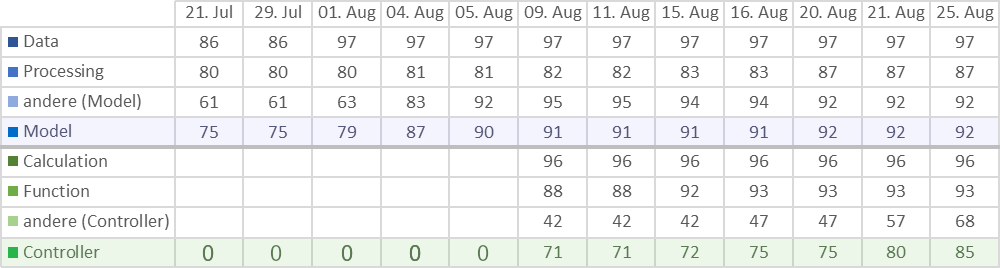
\includegraphics[scale=1.6]{docs/qualityassurance/testreport/img/Table_Coverage.png}}
    \caption{Erfassungsdaten der Testüberdeckung in Prozent}
    \label{fig:sd:Coverage_over_time_data}
\end{figure}

Bei \texttt{andere (Model)} und \texttt{andere (Controller)} handelt es sich um Gruppen an Klassen, die zu keinem Unterpaket zugeordnet sind.
Dessen Werte wurden mithilfe der restlichen Angaben auf das geometrische Mittel geschätzt.\\
Eine graphische Darstellung des zeitlichen Verlaufes wurde anhand der Tabelle erstellt und befindet sich in Abb.~\ref{fig:sd:Coverage_over_time}.

\begin{figure}[H]%
\makebox[0pt]
    {\hspace*{4.8in}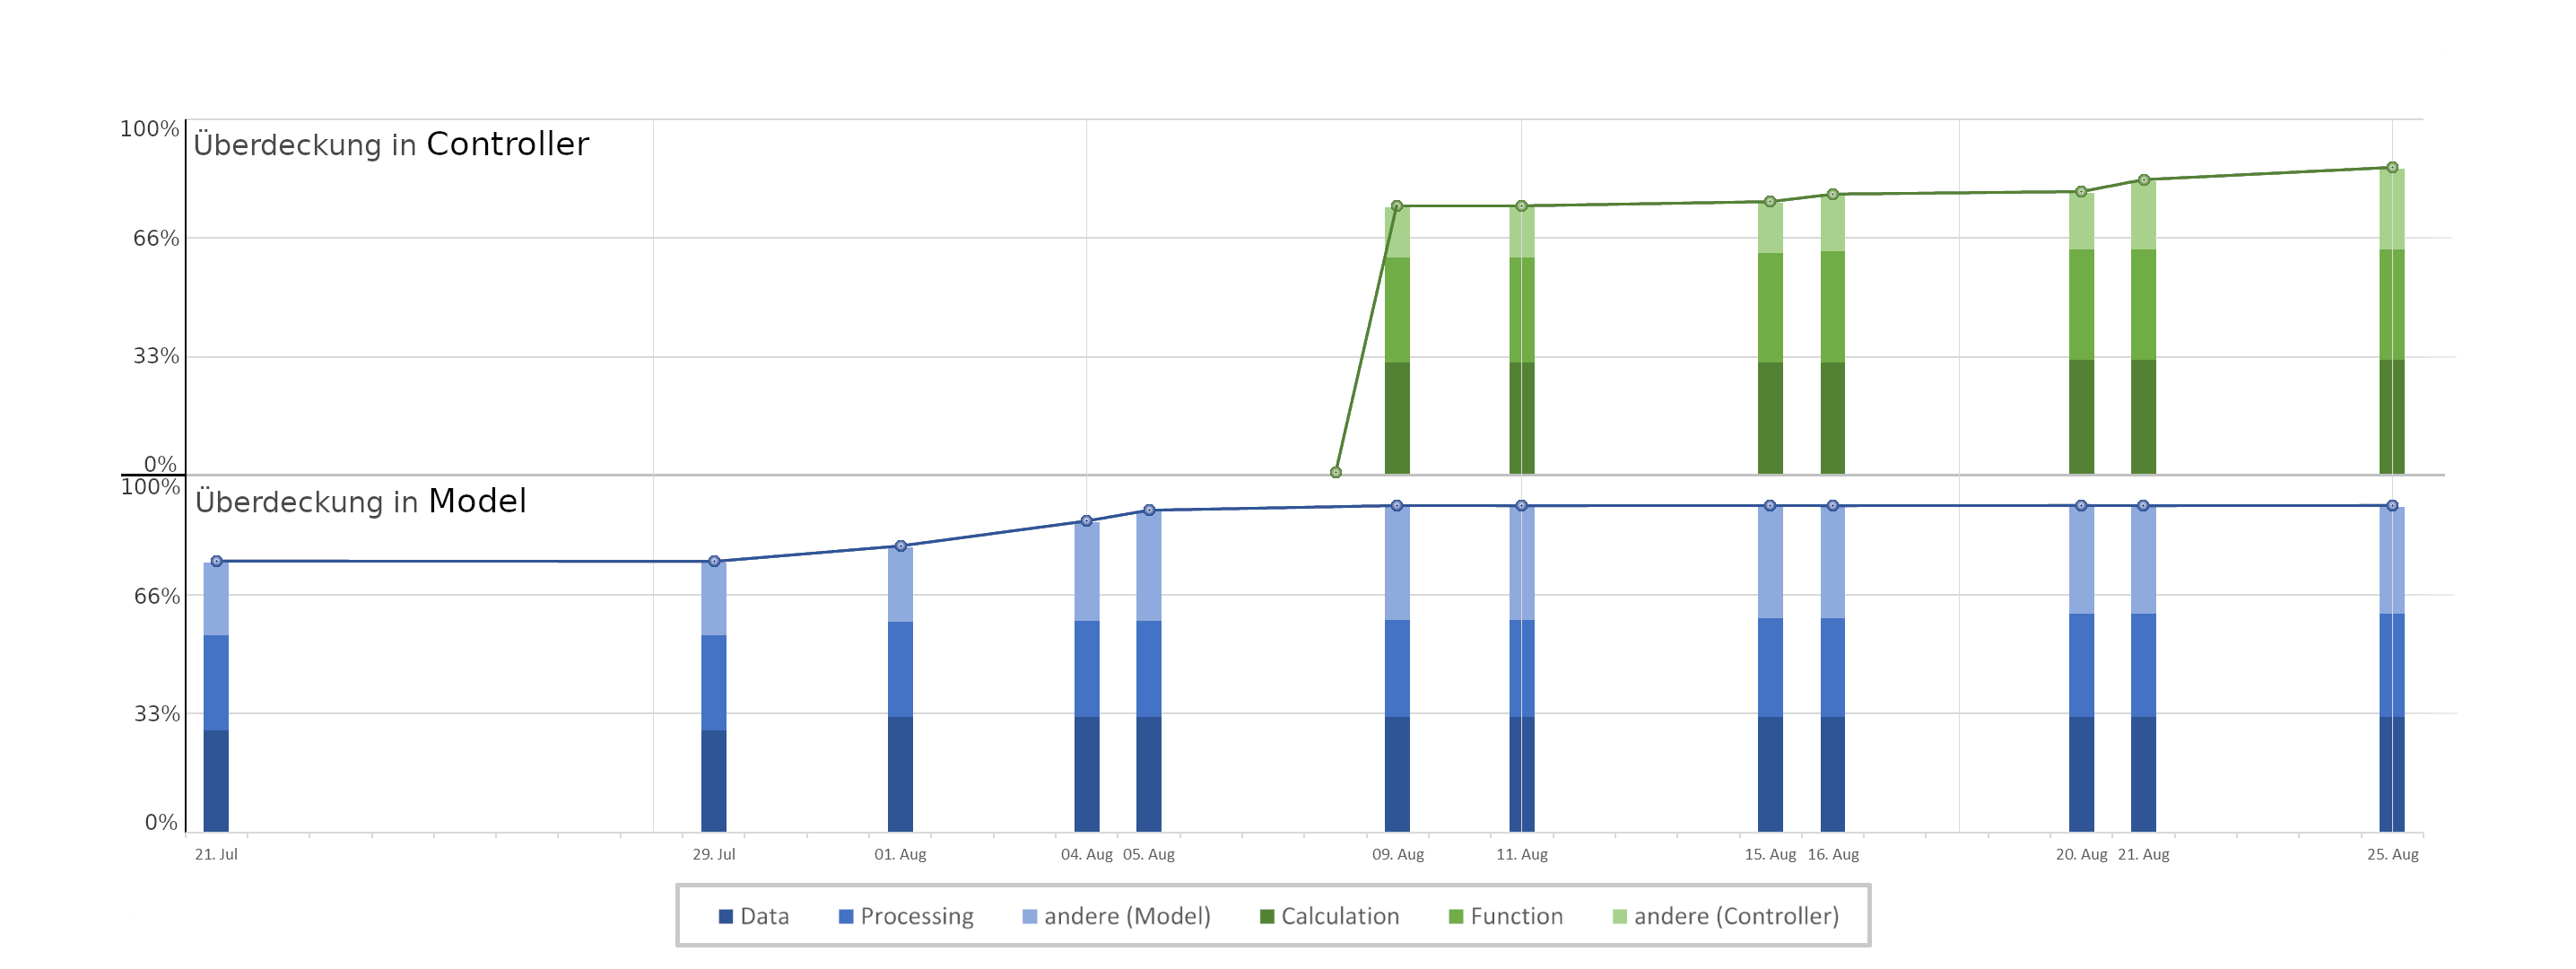
\includegraphics[scale=0.75]{docs/qualityassurance/testreport/img/Diagramm_Coverage.png}}
    \caption{Zeitlicher Verlauf der Testüberdeckung}
    \label{fig:sd:Coverage_over_time}
\end{figure}

Aus der vorangegangenen Phase existierten bereits Testfälle zu den Klassen \classref{SingleLogitBiogemeConfig} und \classref{FunctionalExpression}. Die resultierende Testüberdeckung im \texttt{Model} befand sich somit bereits bei 75~\%.
\\
Zwischen dem 01. und 09. August wurden die restlichen Unit-Tests für das \texttt{Model} erstellt. Hier steigt die Gesamtüberdeckung demnach am deutlichsten. Danach wurden einzelne Testfälle hinzugefügt und verändert, weshalb keine große Änderung der Überdeckung erkennbar ist.
\\
Für die Klassen im \texttt{Controller} wurden am 09. August für die meisten der entsprechenden Klassen Unit-Tests erstellt und die Überdeckung befand sich damit bereits bei 71~\%. Über die restlichen zwei Wochen wurden weitere Testklassen und -fälle hinzugefügt und es sind stetige Anstiege in der Überdeckung erkennbar.
\\
Am Ende der Qualitätssicherungsphase befand sich die Testüberdeckung im \texttt{Model} bei 92~\% und im \texttt{Controller} bei 85~\%. Somit ergibt sich eine Gesamtüberdeckung von über 88~\%. Der angestrebte Bereich wurde demnach erreicht.

\newpage
\subsection{Bugfixes}

Eine weitere Möglichkeit den Verlauf der Phase zu begutachten ist es, die Anzahl erfolgreicher Bugfixes anzuschauen. In Abbildung ~\ref{fig:sd:Overview_of_daily_fixed_bugs_over_time} wird die Anzahl täglich abgeschlossener Bugfixes veranschaulicht. Als abgeschlossen gelten Bugfixes sobald sie als \texttt{Issue} auf Github geschlossen wurden. Abbildung ~\ref{fig:sd:Overview_of_total_fixed_bugs_over_time} gibt eine andere Darstellung an, in welcher die Anzahl neu abgeschlossener Bugfixes an einem Tag anteilig an der Zahl zuvor gelöster Bugs addiert wird. Somit kann ein Gesamtbild des Verlaufes entstehen.
\\

Zu Beginn dieser Phase war es notwendig, sämtliche Tests zu schreiben. Sobald diese Tests durchgeführt wurden, dienten die Ergebnisse dazu, Bugs und Verbesserungspotenziale zu identifizieren. Dies ermöglichte eine gründliche Analyse aller problematischen Bereiche und erleichterte die Suche nach Lösungen.\\

Der hohe Anstieg in Abb.~\ref{fig:sd:Overview_of_daily_fixed_bugs_over_time} am 08. August ist darauf zurückzuführen, dass die Unit-Tests für das Model zwischen dem 01. und dem 09. August fertig gestellt wurden, welche einen großen Teil des Programms abdeckten.\\

Die beschriebene zeitliche Abfolge spiegelt sich auch in den Statistiken wider: In den Anfangsphasen wurden nur wenige Bugs behoben. Erst gegen Ende der Phase ist ein deutlicher Anstieg zu verzeichnen.

\begin{figure}[H]%
    \centering
    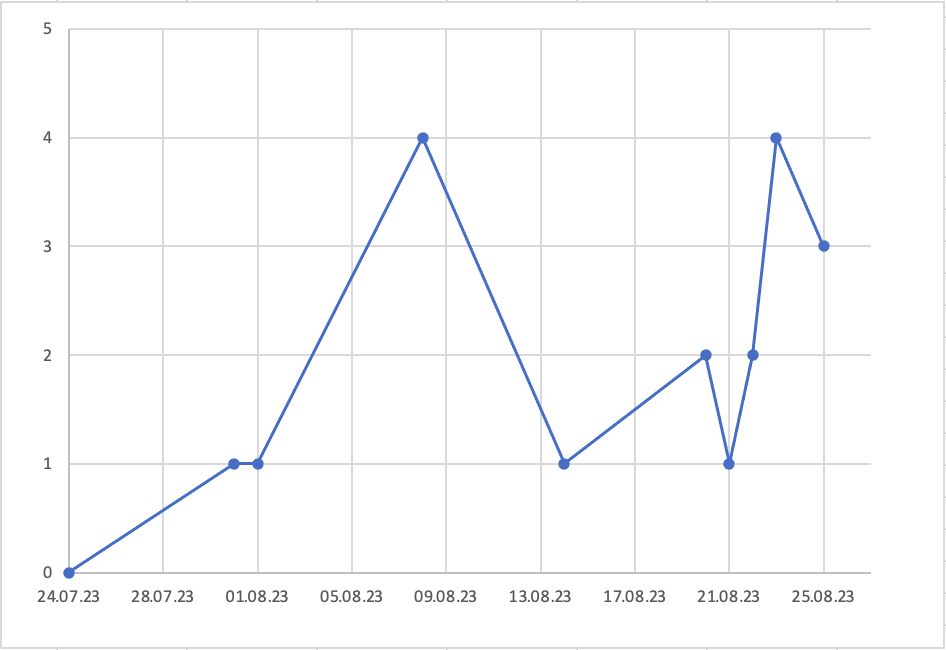
\includegraphics[width=12cm]{docs/qualityassurance/testreport/img/Overview_of_daily_fixed_bugs_over_time.png}
    \caption{Zeitlicher Verlauf der täglichen Bugfixes}
    \label{fig:sd:Overview_of_daily_fixed_bugs_over_time}
\end{figure}
\begin{figure}[H]%
    \centering
    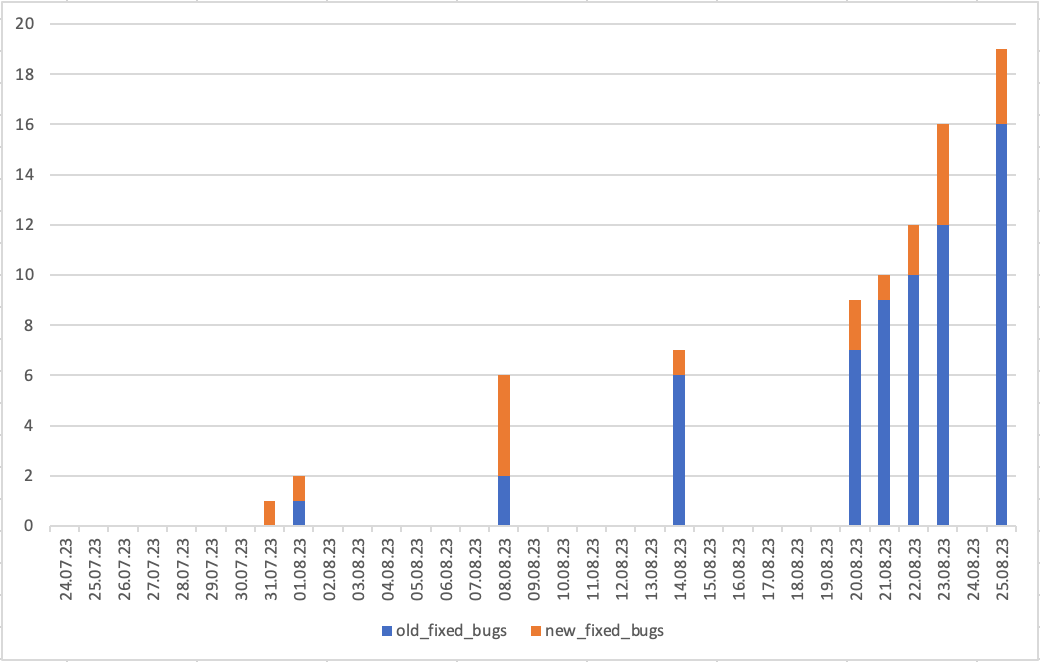
\includegraphics[width=12cm]{docs/qualityassurance/testreport/img/Overview_of_total_fixed_bugs_over_time.png}
    \caption{Zeitlicher Verlauf der Gesamtzahl an Bugfixes}
    \label{fig:sd:Overview_of_total_fixed_bugs_over_time}
\end{figure}

\newpage
\section{Testfälle aus dem Pflichtenheft} \label{testfaelle}

\begin{table}[H]
\begin{tabularx}{\textwidth}{rX}
\vspace{1mm}
\textbf{/T10/}         & \textbf{Importieren der CSV-Datei} \\ \vspace{1mm}
\textbf{Ablauf} & 
    \begin{enumerate}
        \item Gehe zu \guibutton{File} Menu, dann \guibutton{Import Data}
        \item Wähle im File Dialog die Erhebungsdaten (CSV-Datei)
    \end{enumerate} \\ \vspace{1mm}
\textbf{Erfüllt?}  & Ja \\ \vspace{1mm}
\end{tabularx}
\end{table}

\begin{table}[H]
\begin{tabularx}{\textwidth}{rX}
\vspace{1mm}
\textbf{/T11/}         & \textbf{Importieren der Alternativen (Erfolg)} \\ \vspace{1mm}
\textbf{Ablauf} & 
    \begin{enumerate}
        \item Im ModelWidgte, klicke auf \guibutton{Import}
        \item Wähle im File Dialog die Alternative (JSON-Datei)
    \end{enumerate} \\ \vspace{1mm}
\textbf{Erfüllt?}  &  Ja \\ \vspace{1mm}
\end{tabularx}
\end{table}

\begin{table}[H]
\begin{tabularx}{\textwidth}{rX}
\vspace{1mm}
\textbf{/T12/}         & \textbf{Importieren der Alternativen (Teilerfolg)} \\ \vspace{1mm}
\textbf{Ablauf} & 
    \begin{enumerate}
        \item Im ModelWidget klicke auf \guibutton{Import}
        \item Wähle im File Dialog die Alternative (JSON-Datei), welche Fehler enthält.
        \item Es erscheint eine Warn-Dialog. Klicke auf \guibutton{Yes} (Bestätigung des Importierens)
    \end{enumerate} \\ \vspace{1mm}
\textbf{Erfüllt?}  & Ja \\ \vspace{1mm}
\end{tabularx}
\end{table}


\begin{table}[H]
\begin{tabularx}{\textwidth}{rX}
\vspace{1mm}
\textbf{/T13/}         & \textbf{Importieren der Alternativen (Abbruch)} \\ \vspace{1mm}
\textbf{Ablauf} & 
    \begin{enumerate}
        \item Im ModelWidget klicke auf \guibutton{Import}
        \item Wähle im File Dialog die Alternative (JSON-Datei), welche Fehler enthält.
        \item Es erscheint eine Warn-Dialog. Klicke auf \guibutton{Nein} (Abbruch des Importierens)
    \end{enumerate} \\ \vspace{1mm}
\textbf{Erfüllt?}  &  Ja \\ \vspace{1mm}
\end{tabularx}
\end{table}

\begin{table}[H]
\begin{tabularx}{\textwidth}{rX}
\vspace{1mm}
\textbf{/T14/}         & \textbf{Importieren der Attributsableitungen (Erfolg)} \\ \vspace{1mm}
\textbf{Ablauf} & 
    \begin{enumerate}
        \item Im ColumnWidget klicke auf \guibutton{Import}.
        \item Wähle im File Dialog die Ableitung (JSON-Datei).
    \end{enumerate} \\ \vspace{1mm}
\textbf{Erfüllt?}  &  Ja \\ \vspace{1mm}
\end{tabularx}
\end{table}

\begin{table}[H]
\begin{tabularx}{\textwidth}{rX}
\vspace{1mm}
\textbf{/T15/}         & \textbf{Importieren der Attributsableitungen (Teilerfolg)} \\ \vspace{1mm}
\textbf{Ablauf} & 
    \begin{enumerate}
        \item Im ColumnWidget klicke auf \guibutton{Import}.
        \item Wähle im File Dialog die Ableitung (JSON-Datei), welche fehlerhafte Daten enthält.
        \item Es erscheint eine Warn-Dialog. Klicke auf \guibutton{Yes} (Bestätigung des Importierens)
    \end{enumerate} \\ \vspace{1mm}
\textbf{Erfüllt?}  &  Ja\\ \vspace{1mm}
\end{tabularx}
\end{table}

\begin{table}[H]
\begin{tabularx}{\textwidth}{rX}
\vspace{1mm}
\textbf{/T16/}         & \textbf{Importieren der Attributsableitungen (Abbruch)} \\ \vspace{1mm}
\textbf{Ablauf} & 
    \begin{enumerate}
        \item Im ColumnWidget klicke auf \guibutton{Import}.
        \item Wähle im \guibutton{File} Dialog die Ableitung (JSON-Datei), welche fehlerhafte Daten enthält.
        \item Es erscheint eine Warn-Dialog. Klicke auf \guibutton{No} (Abbruch des Importieren)
    \end{enumerate} \\ \vspace{1mm}
\textbf{Erfüllt?}  & Ja \\ \vspace{1mm}
\end{tabularx}
\end{table}

\begin{table}[H]
\begin{tabularx}{\textwidth}{rX}
\vspace{1mm}
\textbf{/T50/}         & \textbf{Exportieren der CSV-Datei (Erfolg)} \\ \vspace{1mm}
\textbf{Ablauf} & 
    \begin{enumerate}
        \item Gehe zu \guibutton{File} Menu, dann zu \guibutton{Export Data}
        \item Wähle im File Dialog den Exportort und Namen der CSV-Datei
    \end{enumerate} \\ \vspace{1mm}
\textbf{Erfüllt?}  & Ja \\ \vspace{1mm}
\end{tabularx}
\end{table}

\begin{table}[H]
\begin{tabularx}{\textwidth}{rX}
\vspace{1mm}
\textbf{/T21/}         & \textbf{Exportieren der CSV-Datei (Teilerfolg)} \\ \vspace{1mm}
\textbf{Ablauf} & 
    \begin{enumerate}
        \item Gehe zu \guibutton{File} Menu, dann zu \guibutton{Export Data}
        \item Wähle im File Dialog den Exportort und Namen der CSV-Datei
        \item Da im Projekt fehlerhafte Informationen sind, erscheint eine Warn-Dialog. Klicke auf \guibutton{Ja} zum Fortfahren.
    \end{enumerate} \\ \vspace{1mm}
\textbf{Erfüllt?}  &  Ja \\ \vspace{1mm}
\end{tabularx}
\end{table}

\begin{table}[H]
\begin{tabularx}{\textwidth}{rX}
\vspace{1mm}
\textbf{/T22/}         & \textbf{Exportieren der CSV-Datei (Abbruch)} \\ \vspace{1mm}
\textbf{Ablauf} & 
\begin{enumerate}
        \item Gehe zu File Menu, dann zu Export Data
        \item Wähle im File Dialog den Exportort und Namen der CSV-Datei
        \item Da im Projekt fehlerhafte Informationen sind, erscheint eine Warndialog. klicke auf Nein zum Abbrechen der Vorgang.
    \end{enumerate} \\ \vspace{1mm}
\textbf{Erfüllt?}  & Ja \\ \vspace{1mm}
\end{tabularx}
\end{table}

\begin{table}[H]
\begin{tabularx}{\textwidth}{rX}
\vspace{1mm}
\textbf{/T23/}         & \textbf{Exportieren der Alternativen (Erfolg)} \\ \vspace{1mm}
\textbf{Ablauf} & 
\begin{enumerate}
        \item Im ModelWidget wähle die zu exportierende Alternative und klicke auf Export
        \item Wähle im File Dialog den Exportort.
    \end{enumerate} \\ \vspace{1mm}
\textbf{Erfüllt?}  &  Ja\\ \vspace{1mm}
\end{tabularx}
\end{table}

\begin{table}[H]
\begin{tabularx}{\textwidth}{rX}
\vspace{1mm}
\textbf{/T24/}         & \textbf{Exportieren der Alternativen (Teilerfolg)} \\ \vspace{1mm}
\textbf{Ablauf} & 
\begin{enumerate}
        \item Im ModelWidget wähle die zu exportierende Alternative und klicke auf Export.
        \item Es erscheint eine Warndialog, weil die gewählte Alternative ungültige Informationen enthält. Klicke auf Ja zum Fortfahren.
        \item Wähle im File Dialog den Exportort.
    \end{enumerate} \\ \vspace{1mm}
\textbf{Erfüllt?}  &  Ja \\ \vspace{1mm}
\end{tabularx}
\end{table}

\begin{table}[H]
\begin{tabularx}{\textwidth}{rX}
\vspace{1mm}
\textbf{/T25/}         & \textbf{Exportieren der Alternativen (Abbruch)} \\ \vspace{1mm}
\textbf{Ablauf} & 
\begin{enumerate}
        \item Im ModelWidget wähle die zu exportierende Alternative und klicke auf Export.
        \item Es erscheint eine Warn-Dialog, weil die gewählte Alternative ungültige Informationen enthält. Klicke auf Nein zum Abbrechen.
    \end{enumerate} \\ \vspace{1mm}
\textbf{Erfüllt?}  &  Ja\\ \vspace{1mm}
\end{tabularx}
\end{table}

\begin{table}[H]
\begin{tabularx}{\textwidth}{rX}
\vspace{1mm}
\textbf{/T26/}         & \textbf{Exportieren der Attributsableitungen (Erfolg)} \\ \vspace{1mm}
\textbf{Ablauf} & 
\begin{enumerate}
        \item Im ColumnWidget wähle die zu exportierende Ableitung und klicke auf Export.
        \item Wähle im File Dialog den Exportort.
    \end{enumerate} \\ \vspace{1mm}
\textbf{Erfüllt?}  &  Ja \\ \vspace{1mm}
\end{tabularx}
\end{table}

\begin{table}[H]
\begin{tabularx}{\textwidth}{rX}
\vspace{1mm}
\textbf{/T27/}         & \textbf{Exportieren der Attributsableitungen (Teilerfolg)} \\ \vspace{1mm}
\textbf{Ablauf} & 
\begin{enumerate}
        \item Im ColumnWidget wähle die zu exportierende Ableitung und klicke auf Export
        \item Da die Ableitung ungültige Angaben enthält, erscheint eine Warndialog. Klicke auf Ja zum Fortfahren.
        \item Wähle im File Dialog den Exportort.
    \end{enumerate} \\ \vspace{1mm}
\textbf{Erfüllt?}  & Ja \\ \vspace{1mm}
\end{tabularx}
\end{table}

\begin{table}[H]
\begin{tabularx}{\textwidth}{rX}
\vspace{1mm}
\textbf{/T28/}         & \textbf{Exportieren der Attributsableitungen (Abbruch)} \\ \vspace{1mm}
\textbf{Ablauf} & 
\begin{enumerate}
        \item Im ColumnWidget wähle die zu exportierende Ableitung und klicke auf Export
        \item Da die Ableitung ungültige Angaben enthält, erscheint eine Warndialog. Klicke auf Nein zum Abbrechen.
    \end{enumerate} \\ \vspace{1mm}
\textbf{Erfüllt?}  & Ja\\ \vspace{1mm}
\end{tabularx}
\end{table}

\begin{table}[H]
\begin{tabularx}{\textwidth}{rX}
\vspace{1mm}
\textbf{/T30/}         & \textbf{Projekt laden} \\ \vspace{1mm}
\textbf{Ablauf} & 
\begin{enumerate}
        \item gehe zu \guibutton{File} Menu, dann \guibutton{Open Project}
        \item Im File Dialog wähle die den Projektpfad.
    \end{enumerate} \\ \vspace{1mm}
\textbf{Erfüllt?}  & Ja \\ \vspace{1mm}
\end{tabularx}
\end{table}

\begin{table}[H]
\begin{tabularx}{\textwidth}{rX}
\vspace{1mm}
\textbf{/T31/}         & \textbf{Projekt speichern (Erfolg)} \\ \vspace{1mm}
\textbf{Ablauf} & 
\begin{enumerate}
        \item gehe zu \guibutton{File} Menu, dann \guibutton{Save Project}
    \end{enumerate} \\ \vspace{1mm}
\textbf{Erfüllt?}  & ja \\ \vspace{1mm}
\end{tabularx}
\end{table}

\begin{table}[H]
\begin{tabularx}{\textwidth}{rX}
\vspace{1mm}
\textbf{/T32/}         & \textbf{Projekt speichern (Erfolg)} \\ \vspace{1mm}
\textbf{Ablauf} & 
\begin{enumerate}
        \item gehe zu \guibutton{File} Menu, dann \guibutton{Save Project}
        \item Da das Projekt ungültige Daten enthält, es erscheint eine Warn Dialog. Klicke auf Ja zum Fortfahren.
    \end{enumerate} \\ \vspace{1mm}
\textbf{Erfüllt?}  & Ja \\ \vspace{1mm}
\end{tabularx}
\end{table}

\begin{table}[H]
\begin{tabularx}{\textwidth}{rX}
\vspace{1mm}
\textbf{/T33/}         & \textbf{Projekt speichern (Abbruch)} \\ \vspace{1mm}
\textbf{Ablauf} & 
\begin{enumerate}
        \item gehe zu \guibutton{File} Menu, dann \guibutton{Save Project}
        \item Da das Projekt ungültige Informationen enthält (invalide Ableitungen oder Alternativen), erscheint ein Warn Dialog. Klicke auf Nein zum Abbrechen der Vorgang
    \end{enumerate} \\ \vspace{1mm}
\textbf{Erfüllt?}  & T33\\ \vspace{1mm}
\end{tabularx}
\end{table}

\begin{table}[H]
\begin{tabularx}{\textwidth}{rX}
\vspace{1mm}
\textbf{/T40/}         & \textbf{Attributsableitung hinzufügen (Erfolg)} \\ \vspace{1mm}
\textbf{Ablauf} &
\begin{enumerate}
    \item Für das Eingeben von Attributsableitungen klicke in ColumnWidget auf \guibutton{+}
    \item Gebe in dem Eingabefenster im \textit{Label}-Feld Name der Ableitung und im \textit{Definiton}-Feld die Ableitung als Funktion.
\end{enumerate} \\ \vspace{1mm}
\textbf{Erfüllt?}  &  
\begin{itemize}
    \item /T40.1/ Intervalle als \texttt{Interval(a, b)} erfüllt
    \item /T40.2/ Gruppen als \texttt{GroupMap()} erfüllt
    \item /T40.3/ Logische Ausdrücke erfüllt
    \item /T40.4/ Vergleiche als \texttt{bool} erkannt erfüllt
\end{itemize}\\ \vspace{1mm}
\end{tabularx}
\end{table}

\begin{table}[H]
\begin{tabularx}{\textwidth}{rX}
\vspace{1mm}
\textbf{/T41/}         & \textbf{Attributsableitung hinzufügen (Misserfolg)} \\ \vspace{1mm}
\textbf{Ablauf} & 
\begin{enumerate}
        \item Für das Eingeben von Attributsableitungen klicke in ColumnWidget auf \guibutton{+}
        \item Gebe in dem Eingabefenster im \textit{Label}-Feld Name der Ableitung und im \textit{Definiton}-Feld die Ableitung als Funktion.
    \end{enumerate} \\ \vspace{1mm}
\textbf{Erfüllt?}  & Nein, die Ableitung wird hinzugefügt, die Fehler werden markiert.  \\ \vspace{1mm}
\end{tabularx}
\end{table}

\begin{table}[H]
\begin{tabularx}{\textwidth}{rX}
\vspace{1mm}
\textbf{/T42/}         & \textbf{Attributsableitung ändern (Erfolg)} \\ \vspace{1mm}
\textbf{Ablauf} & 
\begin{enumerate}
        \item Klicke auf die zu ändernde Funktion.
        \item Ein Textfeld mit der Funktion öffnet sich, es wird eine neue Attributsableitung eingegeben.
        \item Es wird \textit{Enter}-Taste gedrückt.
    \end{enumerate} \\ \vspace{1mm}
\textbf{Erfüllt?}  & Ja  \\ \vspace{1mm}
\end{tabularx}
\end{table}

\begin{table}[H]
\begin{tabularx}{\textwidth}{rX}
\vspace{1mm}
\textbf{/T43/}         & \textbf{Attributsableitung ändern (Misserfolg)} \\ \vspace{1mm}
\textbf{Ablauf} & 
\begin{enumerate}
        \item Klicke auf die zu ändernde Funktion.
        \item Ein Textfeld mit der Funktion öffnet sich, es wird eine neue invalide Attributsableitung eingegeben.
        \item Es wird \textit{Enter}-Tast gedrückt.
    \end{enumerate} \\ \vspace{1mm}
\textbf{Erfüllt?}  & Nein, die invalide Funktion wird übernommen. Fehler werden markiert.  \\ \vspace{1mm}
\end{tabularx}
\end{table}

\begin{table}[H]
\begin{tabularx}{\textwidth}{rX}
\vspace{1mm}
\textbf{/T44/}         & \textbf{Attributsableitung löschen (Erfolg)} \\ \vspace{1mm}
\textbf{Ablauf} & 
\begin{enumerate}
        \item Die zu löschende Funktion wird ausgewählt.
        \item Es wird \guibutton{-} im ColumnWidget gedrückt.
    \end{enumerate} \\ \vspace{1mm}
\textbf{Erfüllt?}  & Ja  \\ \vspace{1mm}
\end{tabularx}
\end{table}

\begin{table}[H]
\begin{tabularx}{\textwidth}{rX}
\vspace{1mm}
\textbf{/T45/}         & \textbf{Attributsableitung löschen (Erfolg)} \\ \vspace{1mm}
\textbf{Ablauf} & 
\begin{enumerate}
        \item Die zu löschende Funktion wird ausgewählt.
        \item Es wird \guibutton{-} im ColumnWidget gedrückt.
    \end{enumerate} \\ \vspace{1mm}
\textbf{Erfüllt?}  & Ja  \\ \vspace{1mm}
\end{tabularx}
\end{table}

\begin{table}[H]
\begin{tabularx}{\textwidth}{rX}
\vspace{1mm}
\textbf{/T46/}         & \textbf{Attributsableitung löschen (Abbruch)} \\ \vspace{1mm}
\textbf{Ablauf} & 
\begin{enumerate}
        \item Die zu löschende Funktion wird ausgewählt.
        \item Es wird \guibutton{-} im ColumnWidget gedrückt.
    \end{enumerate} \\ \vspace{1mm}
\textbf{Erfüllt?}  & Ja  \\ \vspace{1mm}
\end{tabularx}
\end{table}

\begin{table}[H]
\begin{tabularx}{\textwidth}{rX}
\vspace{1mm}
\textbf{/T50/}         & \textbf{Alternative hinzufügen (Erfolg)} \\ \vspace{1mm}
\textbf{Ablauf} & 
\begin{enumerate}
        \item Es wird \guibutton{+} im ModelWidget gedrückt.
        \item Es wird eine valide Alternative eingegeben
    \end{enumerate} \\ \vspace{1mm}
\textbf{Erfüllt?}  & Ja  \\ \vspace{1mm}
\end{tabularx}
\end{table}

\begin{table}[H]
\begin{tabularx}{\textwidth}{rX}
\vspace{1mm}
\textbf{/T50.1/}         & \textbf{Linearkombination hinzufügen} \\ \vspace{1mm}
\textbf{Ablauf} & 
\begin{enumerate}
        \item Es wird \guibutton{+} im ModelWidget gedrückt.
        \item Es wird eine Linearkombination eingegeben.
    \end{enumerate} \\ \vspace{1mm}
\textbf{Erfüllt?}  & Ja  \\ \vspace{1mm}
\end{tabularx}
\end{table}

\begin{table}[H]
\begin{tabularx}{\textwidth}{rX}
\vspace{1mm}
\textbf{/T51/}         & \textbf{Alternative hinzufügen (Misserfolg)} \\ \vspace{1mm}
\textbf{Ablauf} & 
\begin{enumerate}
        \item Es wird \guibutton{+} im ModelWidget gedrückt.
        \item Es wird eine invalide Alternative eingegeben
    \end{enumerate} \\ \vspace{1mm}
\textbf{Erfüllt?}  & Nein, die Alternative wird mit Fehlern hinzugefügt.  \\ \vspace{1mm}
\end{tabularx}
\end{table}

\begin{table}[H]
\begin{tabularx}{\textwidth}{rX}
\vspace{1mm}
\textbf{/T52/}         & \textbf{Alternative ändern (Erfolg)} \\ \vspace{1mm}
\textbf{Ablauf} & 
\begin{enumerate}
        \item Es wird ein Textfeld einer Alternative angeklickt.
        \item Das Textfeld öffnet sich und eine Änderung wird vorgenommen.
    \end{enumerate} \\ \vspace{1mm}
\textbf{Erfüllt?}  & Ja \\ \vspace{1mm}
\end{tabularx}
\end{table}

\begin{table}[H]
\begin{tabularx}{\textwidth}{rX}
\vspace{1mm}
\textbf{/T53/}         & \textbf{Alternative ändern (Misserfolg)} \\ \vspace{1mm}
\textbf{Ablauf} & 
\begin{enumerate}
        \item Es wird ein Textfeld einer Alternative angeklickt.
        \item Das Textfeld öffnet sich und eine Änderung wird vorgenommen.
    \end{enumerate} \\ \vspace{1mm}
\textbf{Erfüllt?}  & Nein, die Alternative wird geändert. Der Nutzer bekommt den Fehler angezeigt. \\ \vspace{1mm}
\end{tabularx}
\end{table}

\begin{table}[H]
\begin{tabularx}{\textwidth}{rX}
\vspace{1mm}
\textbf{/T54/}         & \textbf{Alternative löschen} \\ \vspace{1mm}
\textbf{Ablauf} & 
\begin{enumerate}
        \item Es wird eine Alternative ausgewählt.
        \item Es wird \guibutton{-} im ModelWidget gedrückt.
    \end{enumerate} \\ \vspace{1mm}
\textbf{Erfüllt?}  & Ja \\ \vspace{1mm}
\end{tabularx}
\end{table}

\begin{table}[H]
\begin{tabularx}{\textwidth}{rX}
\vspace{1mm}
\textbf{/T60/}         & \textbf{Berechnung durchführen (Erfolg)} \\ \vspace{1mm}
\textbf{Ablauf} & 
\begin{enumerate}
        \item Es wird \guibutton{Calculate Evaluation} gedrückt.
    \end{enumerate} \\ \vspace{1mm}
\textbf{Erfüllt?}  & Ja \\ \vspace{1mm}
\end{tabularx}
\end{table}

\begin{table}[H]
\begin{tabularx}{\textwidth}{rX}
\vspace{1mm}
\textbf{/T61/}         & \textbf{Berechnung durchführen (Teilerfolg)} \\ \vspace{1mm}
\textbf{Ablauf} & 
\begin{enumerate}
        \item Es wird \guibutton{Calculate Evaluation} gedrückt.
    \end{enumerate} \\ \vspace{1mm}
\textbf{Erfüllt?}  & Nein, nicht existente Variablen in den Alternativen werden als Betas berechnet. Die Availability Conditions dürfen nicht invalide sein. \\ \vspace{1mm}
\end{tabularx}
\end{table}

\begin{table}[H]
\begin{tabularx}{\textwidth}{rX}
\vspace{1mm}
\textbf{/T62/}         & \textbf{Berechnung durchführen (Abbruch)} \\ \vspace{1mm}
\textbf{Ablauf} & 
\begin{enumerate}
        \item Es wird \guibutton{Calculate Evaluation} gedrückt.
    \end{enumerate} \\ \vspace{1mm}
\textbf{Erfüllt?}  & Nein, der Nutzer bekommt Meldung was invalide ist. Die Berechnung wird nicht gestartet. \\ \vspace{1mm}
\end{tabularx}
\end{table}

\begin{table}[H]
\begin{tabularx}{\textwidth}{rX}
\vspace{1mm}
\textbf{/T63/}         & \textbf{Berechnung durchführen (Abbruch)} \\ \vspace{1mm}
\textbf{Ablauf} & 
\begin{enumerate}
        \item Es wird \guibutton{Calculate Evaluation} gedrückt.
    \end{enumerate} \\ \vspace{1mm}
\textbf{Erfüllt?}  & Nein, es gibt keine Funktion, die die Berechnungen abbricht. Da diese weniger Zeitaufwand als erwartet haben, wurde diese Funktion nicht implementiert. \\ \vspace{1mm}
\end{tabularx}
\end{table}

\begin{table}[H]
\begin{tabularx}{\textwidth}{rX}
\vspace{1mm}
\textbf{/T64/}         & \textbf{Exportieren der Ergebnisse} \\ \vspace{1mm}
\textbf{Ablauf} & 
\begin{enumerate}
        \item Es wird \guibutton{Export Evaluation} gedrückt.
    \end{enumerate} \\ \vspace{1mm}
\textbf{Erfüllt?}  & Ja \\ \vspace{1mm}
\end{tabularx}
\end{table}

\begin{table}[H]
\begin{tabularx}{\textwidth}{rX}
\vspace{1mm}
\textbf{/T70/}         & \textbf{Änderung der Schwellwerte} \\ \vspace{1mm}
\textbf{Ablauf} & 
\begin{enumerate}
        \item Es wird \guibutton{View Options} im Evaluation Widget gedrückt.
        \item Es werden Schwellwerte eingestellt.
        \item Es wird \guibutton{Apply Thresholds} gedrückt.
    \end{enumerate} \\ \vspace{1mm}
\textbf{Erfüllt?}  & Ja \\ \vspace{1mm}
\end{tabularx}
\end{table}

\begin{table}[H]
\begin{tabularx}{\textwidth}{rX}
\vspace{1mm}
\textbf{/T80/}         & \textbf{Erweiterbarkeit} \\ \vspace{1mm}
\textbf{Erfüllt?}  & Nein, es liegt keine Optimierungsmöglichkeit vor. \\ \vspace{1mm}
\end{tabularx}
\end{table}


\newpage
\section{Auswertung Usertests} \label{usertests}
\subsection{Probleme am Programm}

\subsubsection*{Import Data schwer zu finden}
\begin{tabular}{ll}
\begin{tabularx}{\textwidth}{rX}
    \textbf{Beschreibung:} & \guibutton{Import Data} wurde nicht schnell gefunden und oft mit \\
    & Open Project, Import von Ableitungen oder \\
    & Nutzenfunktionen verwechselt. \\
    \textbf{Priorität:} & hoch\\
    \textbf{Ursache:} & Die Operation ist versteckt im Dateimenü \\
    \textbf{Verbesserungsvorschlag:} & Eine Programmanleitung bereitstellen \\
    \textbf{Wurde verbessert?} & Ja\\
      \end{tabularx}
\end{tabular}

\subsubsection*{Erläuterung der Syntax fehlt}
\begin{tabular}{ll}
\begin{tabularx}{\textwidth}{rX}
    \textbf{Beschreibung:} & Syntax für Ableitung oder Nutzenfunktion nicht intuitiv genug.\\
    \textbf{Priorität:} & mittel\\
    \textbf{Ursache:} & Keine Erläuterung der Syntax vorhanden\\
    \textbf{Verbesserungsvorschlag:} & Eine Programmanleitung erstellen\\
    \textbf{Wurde verbessert?} & Ja\\
    \end{tabularx}
\end{tabular}

\subsubsection*{Eingabeknöpfe für Ableitungen und Nutzenfunktionen nicht leicht zu finden}
\begin{tabular}{ll}
\begin{tabularx}{\textwidth}{rX}
    \textbf{Beschreibung:} & Eingabeknöpfe für Ableitungen und Nutzenfunktionen wurden  \\
    &miteinader oft verwechselt. Sie sind auf dem \\
    & ersten Blick nicht unterscheidbar. \\
    \textbf{Priorität:} & niedrig\\
    \textbf{Ursache:} & Keine genaue Beschreibung Rollen der einzelenen \\
    & Teile(Widgets) des Programms.\\
    \textbf{Verbesserungsvorschlag:} & Einführung von Tooltips \\
    \textbf{Wurde verbessert?} & Ja\\
    \end{tabularx}
\end{tabular}

\subsubsection*{Fehlermeldungen unklar}
\begin{tabular}{ll}
\begin{tabularx}{\textwidth}{rX}
    \textbf{Beschreibung:} & Fehlerursache im Fehlermeldungen werden nicht genug erläutert  \\
    \textbf{Priorität:} & hoch\\
    \textbf{Ursache:} & Fehlersuche wird mit builtin Funktion eval() ausgeführt. \\
    & Diese liefert oft ungenaue Erklärungen, z.~B. nur dass es eine invalide Syntax gibt, aber nicht was invalide ist.\\
    \textbf{Verbesserungsvorschlag:} & Häufige Fehlerursachen mit besseren Fehlerbeschreibungen in der Konfiguration hartkodieren. \\
    \textbf{Wurde verbessert?} & Nein\\
\end{tabularx}
\end{tabular}

\subsubsection*{Evaluation und Processing Widgets unklar}
\begin{tabular}{ll}
\begin{tabularx}{\textwidth}{rX}
    \textbf{Beschreibung:} & Unterschied zwischen Evaluation und Processing Widgets \\
    & auf dem ersten Blick nicht klar.\\
    \textbf{Priorität:} & niedrig\\
    \textbf{Ursache:} & Keine genaue Beschreibung Rollen der einzelenen \\
    & Teile(Widgets) des Programms.\\
    \textbf{Verbesserungsvorschlag:} & Programmanleitung erstellen\\
    \textbf{Wurde verbessert?} & Ja\\
    \end{tabularx}
\end{tabular}

\subsubsection*{ThresholdWindow nicht leicht zu finden}
\begin{tabular}{ll}
\begin{tabularx}{\textwidth}{rX}
    \textbf{Beschreibung:} & ThresholdWindow für Eingabe der Schwellwerte \\
    & nicht vom ersten Blick auffindbar\\
    \textbf{Priorität:} & niedrig\\
    \textbf{Ursache:} & Knopf \guibutton{View Options} konnte bei jedem Nutzer\\
    &  eine andere Bedeutung haben.\\
    \textbf{Verbesserungsvorschlag:} & \guibutton{View Options} Knopf umbennenen. \\
    \textbf{Wurde verbessert?} & Ja\\
    \end{tabularx}
\end{tabular}

\subsubsection*{Fehler bei Eingaben im ModelWidgets nicht leicht sichtbar}
\begin{tabular}{ll}
\begin{tabularx}{\textwidth}{rX}
    \textbf{Beschreibung:} & Fehler bei Definition einer Nutzenfunktion \\
    & wird bei langen Eingaben versteckt. \\
    \textbf{Priorität:} & niedrig\\
    \textbf{Ursache:} & Spalten werden mit Länge der Eingabe \\
    &  bzw. Bei Fehlern nicht erweitert. \\
    \textbf{Verbesserungsvorschlag:} & Hintergrundfarbe der fehlerhaften Funktion ändert sich. \\
    \textbf{Wurde verbessert?} & Ja \\
    \end{tabularx}
\end{tabular}

\subsubsection*{Fenster ist zu klein um Funktionen vollständig anzuzeigen}
\begin{tabular}{ll}
\begin{tabularx}{\textwidth}{rX}
    \textbf{Beschreibung:} & Nutzer konnten die Funktionen nicht vollständig lesen und baten um größere Fenster.\\
    \textbf{Priorität:} & niedrig\\
    \textbf{Ursache:} & Es wird immer die Standardeinstellung verwendet. \\
    \textbf{Verbesserungsvorschlag:} & Standardeinstellung durch größere überschreiben.\\
    \textbf{Wurde verbessert?} & Nein\\
    \end{tabularx}
\end{tabular}

\subsubsection*{Eine Zeile für die Eingabe von Funktionen zu wenig Patz}
\begin{tabular}{ll}
\begin{tabularx}{\textwidth}{rX}
    \textbf{Beschreibung:} &Nutzer brauchten mehr Platz für die Eingabe von Funktionen und wollten die gesamte Funktion sichtbar haben.\\
    \textbf{Priorität:} & mittel\\
    \textbf{Ursache:} & Es wurde nur eine Zeile für die Funktionseingabe vorgesehen. \\
    \textbf{Verbesserungsvorschlag:} & Es gibt ein ganzes Textfeld für die Funktionseingabe.\\
    \textbf{Wurde verbessert?} & Ja\\
    \end{tabularx}
\end{tabular}

\subsubsection*{Verwendung der Variablennamen in den Funktionen schwer}
\begin{tabular}{ll}
\begin{tabularx}{\textwidth}{rX}
    \textbf{Beschreibung:} & Nutzer haben während der Eingabe keinen Überblick über die möglichen verwendbaren Variablen, und müssen diese Labels ohne Hilfe korrekt eingeben, damit Funktionen richtig definiert sind.\\
    \textbf{Priorität:} & mittel\\
    \textbf{Ursache:} & Keine gute Variablenübersicht im Eingabefenster. \\
    \textbf{Verbesserungsvorschlag:} & Autocomplete der Variablen in der Funktionseingabe.\\
    \textbf{Wurde verbessert?} & Nein\\
    \end{tabularx}
\end{tabular}

\subsubsection*{Fehlermeldung eines Fehlerhaften Choice Index nicht verständlich}
\begin{tabular}{ll}
\begin{tabularx}{\textwidth}{rX}
    \textbf{Beschreibung:} & Sind nicht alle Choice Indizes von 0 bis n-1 vorhanden kann die Berechnung nicht durchgeführt werden. Die Fehlermeldung ist nicht verständlich, und weißt nicht darauf hin, wie die Choice Indizes funktionieren.\\
    \textbf{Priorität:} & mittel\\
    \textbf{Ursache:} & Es wird nur die von Python gelieferte Fehlermeldung ausgegeben und die Verwendung der Indizes nicht erklärt. \\
    \textbf{Verbesserungsvorschlag:} & Erklärung der Choice Indizes in der Syntax sowie im \emph{User Manual}.\\
    \textbf{Wurde verbessert?} & Ja\\
    \end{tabularx}
\end{tabular}

\subsubsection*{Unklar ob Berechnung läuft}
\begin{tabular}{ll}
\begin{tabularx}{\textwidth}{rX}
    \textbf{Beschreibung:} & Wenn der Knopf zum Start der Berechnung gedrückt wird passiert nichts und die Nutzer haben den Knopf mehrfach gedrückt.\\
    \textbf{Priorität:} & hoch\\
    \textbf{Ursache:} & Es gibt keine Anzeige ob eine Berechnung läuft. \\
    \textbf{Verbesserungsvorschlag:} & Anzeige, dass Berechnung läuft.\\
    \textbf{Wurde verbessert?} & Nein\\
    \end{tabularx}
\end{tabular}

\subsubsection*{Unklar was mit "Definition" gemeint}
\begin{tabular}{ll}
\begin{tabularx}{\textwidth}{rX}
    \textbf{Beschreibung:} & Im Eingabe Fenster für die Funktionen gibt es unter anderem die Felder \emph{Label} und \emph{Definition}. Nutzer wussten nicht was in diese eingegeben werden soll.\\
    \textbf{Priorität:} & hoch\\
    \textbf{Ursache:} & Keine Erklärung der Felder. \\
    \textbf{Verbesserungsvorschlag:} & Nutzeranleitung und Infofeld.\\
    \textbf{Wurde verbessert?} & Ja\\
    \end{tabularx}
\end{tabular}

\subsubsection*{Markierung verschwindet bei der Bearbeitung von den Funktionen}
\begin{tabular}{ll}
\begin{tabularx}{\textwidth}{rX}
    \textbf{Beschreibung:} & In den Tabellen ist die Fehlermarkierung in den Funktionen nur sichtbar wenn diese nicht bearbeitet werden.\\
    \textbf{Priorität:} & mittle\\
    \textbf{Ursache:} & Die Fehlermarkierung verschwindet in dem Moment wo die Bearbeitung beginnt. \\
    \textbf{Verbesserungsvorschlag:} & Anzeigen der Fehler während der Bearbeitung, oder Öffnen eines separaten Bearbeitungsfensters mit mehr Platz zur Fehlerübersicht.\\
    \textbf{Wurde verbessert?} & Nein\\
    \end{tabularx}
\end{tabular}

\subsubsection*{Betas der Alternativen nicht erkennbar}
\begin{tabular}{ll}
\begin{tabularx}{\textwidth}{rX}
    \textbf{Beschreibung:} & In der Tabelle der Alternativen werden die Betas der Nutzenfunktionen implizit darüber definiert, dass alle unbekannten Variablen als Betas berechnet werden. Die Nutzer müssen selber aufmerksam sein, was berechnet wird.\\
    \textbf{Priorität:} & mittle\\
    \textbf{Ursache:} & Keine Markierung der Betas. \\
    \textbf{Verbesserungsvorschlag:} & Markierung der Betas mit einer anderen Farbe als die Fehler.\\
    \textbf{Wurde verbessert?} & Nein\\
\end{tabularx}
\end{tabular}


\subsection{Wünsche der Nutzer}

\subsubsection*{Mehr Optionen für die Schwellwerte gewünscht}
\begin{tabular}{ll}
\begin{tabularx}{\textwidth}{rX}
    \textbf{Beschreibung:} & Es ist nur möglich Schwellwerte einzustellen, die ein absolutes Minimum sind. Die Nutzer wünschten sich die Möglichkeiten auch Beträge oder Maxima als Schwellwerte einzustellen.\\
    \textbf{Priorität:} & niedrig\\
    \textbf{Ursache:} & Ist nicht im Pflichtenheft gefordert worden. \\
    \textbf{Verbesserungsvorschlag:} & Erweiterung der Funktionen des Schwellwert Fensters.\\
    \textbf{Wurde verbessert?} & Nein\\
    \end{tabularx}
\end{tabular}

\subsubsection*{Mehr Werte bzw. Ergebnisse}
\begin{tabular}{ll}
\begin{tabularx}{\textwidth}{rX}
    \textbf{Beschreibung:} & Es werden nur die im Pflichtenheft beschriebenen Ergebnisse ausgegeben. Nutzer wollten alle berechenbare Werte angezeigt bekommen.\\
    \textbf{Priorität:} & niedrig\\
    \textbf{Ursache:} & Ist nicht im Pflichtenheft gefordert worden. \\
    \textbf{Verbesserungsvorschlag:} & Erweiterung der Ergebnisausgabe.\\
    \textbf{Wurde verbessert?} & Nein\\
    \end{tabularx}
\end{tabular}

\subsubsection*{Vergleich von Ergebnissen verschiedener Modelle}
\begin{tabular}{ll}
\begin{tabularx}{\textwidth}{rX}
    \textbf{Beschreibung:} & Nutzer wollen die geänderten Ergebnisse nach Änderungen im Modell vergleichen.\\
    \textbf{Priorität:} & niedrig\\
    \textbf{Ursache:} & Ist nicht im Pflichtenheft gefordert worden. \\
    \textbf{Verbesserungsvorschlag:} & Option zum Vergleich von gespeicherten Ergebnistabellen implementieren.\\
    \textbf{Wurde verbessert?} & Nein\\
    \end{tabularx}
\end{tabular}

\newpage
\section{Bugs} \label{bugs}

\subsubsection*{Zyklische Definitionen führen zum Programmabsturz}
\begin{tabular}{ll}
    \textbf{Benutztes Werkzeug:} & Monkey-Testing\\
    \textbf{Priorität:} & hoch\\
    \textbf{Fehlersymptom:} & Programmabsturz bei einer zyklischen Definition\\
    \textbf{Fehlerursache:} & Unzureichende Kommunikation über Implementierungsort\\
    & während der Implementierungsphase. \\
    \textbf{Fehlerbehebung:} & Ausdrucksauswertung wurde an einer Stelle vereinigt.\\
    \textbf{Wurde behoben?:} & Ja\\
\end{tabular}

\subsubsection*{Zusätzliches Symbol in Fehlermeldungen}
\begin{tabular}{ll}
    \textbf{Benutztes Werkzeug:} & Monkey-Testing\\
    \textbf{Priorität:} & niedrig\\
    \textbf{Fehlersymptom:} & Fehlernachrichten umfassen zusätzlich das Symbol nach dem Fehler\\
    \textbf{Fehlerursache:} & Unnötige Erhöhung des Offsets\\
    \textbf{Fehlerbehebung:} & Codestelle finden und Offset reduzieren\\
    \textbf{Wurde Behoben?:} & Ja\\
\end{tabular}

\subsubsection*{Verschobene Markierung bei Fehlern}
\begin{tabular}{ll}
    \textbf{Benutztes Werkzeug:} & Monkey-Testing\\
    \textbf{Priorität:} & mittel\\
    \textbf{Fehlersymptom:} & Farbliche Markierung von Fehlern für Windows-Systeme verschoben\\
    \textbf{Fehlerursache:} & Verschiebung von Parametern des Betriebssystems abhängig\\
    \textbf{Fehlerbehebung:} & Unterscheidung des Offsets nach Betriebssystem\\
    \textbf{Wurde Behoben?:} & Ja\\
\end{tabular}

\subsubsection*{Undo nach dem Löschen von Eingaben unkorrekt}
\begin{tabular}{ll}
    \textbf{Benutztes Werkzeug:} & Monkey Testing\\
    \textbf{Priorität:} & hoch\\
    \textbf{Fehlersymptom:} & Wird eine Ableitung aus einem bereits existierenden Projekt gelöscht\\
    &und mit \guibutton{Undo} wiederhergestellt, so erscheint die Ableitung \\
    &wieder, aber ihre JSON-Datei wird ohne explizites Speichern \\
    & nicht wieder hergestellt.\\
    \textbf{Fehlerursache:} & Das Projekt wird nach Ausführung von \guibutton{Undo} nicht gespeichert.\\
    \textbf{Fehlerbehebung:} & Speicherabfrage vor dem Schließen des Projektes nach Änderungen.\\
    \textbf{Wurde Behoben?:} & Ja\\
\end{tabular}

\subsubsection*{Widerrufen/Wiederholen-Funktion funktioniert in einem Bereich nicht}
\begin{tabular}{ll}
    \textbf{Benutztes Werkzeug:} & Unit-Test\\
    \textbf{Priorität:} & hoch\\
    \textbf{Fehlersymptom:} & Widerrufen/Wiederholen-Funktion funktioniert nicht\\
    & für die Verarbeitungseinstellungen\\
    \textbf{Fehlerursache:} & Beim Anlegen eines neuen \texttt{ProjectSnapshot} wurde die Liste \\
    & mit allen Verarbeitungskonfigurationen nicht neu angelegt,\\
    & sodass sie im Speicher noch mit dem vorherigen Snapshot verknüpft war.\\
    \textbf{Fehlerbehebung:} & Liste wird nun kopiert, bevor diese durch\\
    & \texttt{set\_config\_settings} modifiziert wird.\\
    \textbf{Wurde Behoben?:} & Ja\\
\end{tabular}

%Issue #80
\subsubsection*{Export Data funktioniert nicht}
\begin{tabular}{ll}
    \textbf{Benutztes Werkzeug:} & Monkey Testing\\
    \textbf{Priorität:} & hoch\\
    \textbf{Fehlersymptom:} & Export Data erstellt keine CSV-Datei im vorgegebenem Verzeichnis.\\
    \textbf{Fehlerursache:} & Falsche Konfiguration der Erhebungsdaten.\\
    \textbf{Fehlerbehebung:} & Auswertung der Erhebungsdaten repariert.\\
    \textbf{Wurde Behoben?:} & Ja\\
\end{tabular}

\subsubsection*{EvaluationWidget bleibt unverändert}
\begin{tabular}{ll}
    \textbf{Benutztes Werkzeug:} & Monkey Testing\\
    \textbf{Priorität:} & hoch\\
    \textbf{Fehlersymptom:} & Wird ein neues Projekt geöffnet, so bleibt die \\
    & Auswertung aus dem vorherigen Projekt im Programm sichtbar.\\
    \textbf{Fehlerursache:} & Falsche Methode \texttt{QTableView.clearSelection()} eingesetzt, \\
    & da ihr Zweck falsch verstanden wurde. \\
    \textbf{Fehlerbehebung:} & Statt \texttt{clearSelection()}  wird eine leere \texttt{DataFrame} in \texttt{QTableView}\\
    & eingesetzt. Somit erscheint die Tabelle im EvaluationWidget leer.\\
    \textbf{Wurde Behoben?:} & Ja\\
\end{tabular}

%Issue 56
\subsubsection*{Fehlermarkierung fehlt bei den Variablen im ProcessingWidget}
\begin{tabular}{ll}
    \textbf{Benutztes Werkzeug:} & Monkey-Testing\\
    \textbf{Priorität:} & hoch\\
    \textbf{Fehlersymptom:} & Die im ProcessingWidget definierten Variablen sind\\
    & ohne Markierung vorhandener Fehler dargestellt.\\
    \textbf{Fehlerursache:} & Implementierung wurde vergessen.\\
    \textbf{Fehlerbehebung:} & Implementierung wurde nachgeholt.\\
    \textbf{Wurde Behoben?:} & Ja\\
\end{tabular}

%Issue #101
\subsubsection*{Problem beim Laden eines Projekts mit ProcessingWidget-Variablen}
\begin{tabular}{ll}
    \textbf{Benutztes Werkzeug:} & Monkey-Testing\\
    \textbf{Priorität:} & hoch\\
    \textbf{Fehlersymptom:} & Exception beim Laden eines Projekts mit Variablen im ProcessingWidget.\\
    \textbf{Fehlerursache:} & Beim einlesen der Variablen wird anstatt einer \classref{FunctionalExpression}\\
    & lediglich ein \classref{str} (String) des Ausdrucks Programmspeicher hinterlegt\\
    & (falscher Datentyp).\\
    \textbf{Fehlerbehebung:} & Der eingelesene Datentyp wurde korrigiert.\\
    \textbf{Wurde Behoben?:} & Ja\\
\end{tabular}

%Issue #104
\subsubsection*{Konfigurationsvariablen werden beim Laden falsch zugeordnet}
\begin{tabular}{ll}
    \textbf{Benutztes Werkzeug:} & Monkey-Testing\\
    \textbf{Priorität:} & hoch\\
    \textbf{Fehlersymptom:} & Die im \classref{ProcessingWidget} definierten Konfigurationsvariablen werden\\
    & nach dem Speichern und erneuten Öffnen des Projekts einer anderen\\
    & Konfiguration zugeordnet und nicht in derjenigen, in der sie definiert wurden.\\
    \textbf{Fehlerursache:} & Die Konfigurationseinstellungen werden beim Speichern in einem\\
    & Ordner gespeichert, der den Namen der jeweiligen Konfiguration trägt.\\
    & Beim einlesen wird dieses Verzeichnis von Oben nach Unten durchgegangen\\
    & und entsprechend der Einlesereihenfolge einer Konfiguration zugeordet.\\
    & Dies führt dazu, dass nach dem Einlesen möglicherweise eine andere\\
    & Konfiguration die Einstellungen aus einem Ordner erhält, als dies\\
    & gespeichert wurde.\\
    \textbf{Fehlerbehebung:} & Die Verzeichnisse werden nun mit einem numerischen Index benannt,\\
    &sodass die gleiche Zuordnung beim Speichern und Lesen sichergestellt ist.\\
    \textbf{Wurde Behoben?:} & Ja\\
\end{tabular}

%Issue #105
\subsubsection*{Definitionstabelle im ProcessingWidget aktualisiert sich nicht}
\begin{tabular}{ll}
    \textbf{Benutztes Werkzeug:} & Monkey-Testing\\
    \textbf{Priorität:} & hoch\\
    \textbf{Fehlersymptom:} & Die Tabelle im \classref{ProcessingWidget} zur Definition von Variablen\\
    & aktualisiert sich nicht, wenn der Nutzer eine andere \\
    &Konfiguration auswählt.\\
    \textbf{Fehlerursache:} & Benutzeroberfläche wird nach Auswahl einer neuen Konfiguration\\
    & nicht aktualisiert.\\
    \textbf{Fehlerbehebung:} & Aktualisierungsfunktion wird nach Auswahl einer Konfiguration aufgerufen.\\
    \textbf{Wurde Behoben?:} & Ja\\
\end{tabular}

\subsubsection*{Save Project As speichert nicht den Dateipfad}
\begin{tabular}{ll}
    \textbf{Benutztes Werkzeug:} & Monkey-Testing\\
    \textbf{Priorität:} & mittel\\
    \textbf{Fehlersymptom:} & Projekte, die über \guibutton{Save Project As} gespeichert werden, werden\\
    & danach weiterhin als nicht-gespeichert behandelt.\\
    & Speichern über \guibutton{Save} erfordert erneut Eingabe des Dateipfades.\\
    \textbf{Fehlerursache:} & Fehlendes Sichern des Pfades nach Speicherung.\\
    \textbf{Fehlerbehebung:} & Dateipfad nach Speicherung setzen.\\
    \textbf{Wurde Behoben?:} & Ja\\
\end{tabular}

\subsubsection*{Spalten ändern Breite nach jeder Aktion}
\begin{tabular}{ll}
    \textbf{Benutztes Werkzeug:} & Monkey-Testing\\
    \textbf{Priorität:} & hoch\\
    \textbf{Fehlersymptom:} & Spaltenbreiten des Column und Modelwidgets ändern sich bei jeder\\
    & Aktion.\\
    \textbf{Fehlerursache:} & Column- und Modelwidgets setzen nach jedem Aufruf von \texttt{update()}\\
    & die Spaltenbreite auf den Standardwert zurück.\\
    \textbf{Fehlerbehebung:} & Aktuelle Spaltenbreite wird vor dem Update ausgelesen und nach\\
    & dem Update erneut angewandt.\\
    \textbf{Wurde behoben?:} & Ja\\
\end{tabular}

\subsubsection*{Attributsableitungen werden nach jeder Änderung nach ober gescrollt}
\begin{tabular}{ll}
    \textbf{Benutztes Werkzeug:} & Monkey-Testing\\
    \textbf{Priorität:} & hoch\\
    \textbf{Fehlersymptom:} & Nach jeder Aktion ist das ColumnWidget wieder zurückgesetzt auf den\\
    &Stand dass die oberste Funktion angezeigt wird und die zuletzt \\
    &hinzugefügten Funkionen verschwinden aus dem Blick.\\
    \textbf{Fehlerursache:} & Das ist die Standardeinstellung.\\
    \textbf{Fehlerbehebung:} & Nach jeder Aktion wird nach unten gescrollt, sodass die letzte\\
    & hinzugefügte Funktion sichtbar ist.\\
    \textbf{Wurde behoben?:} & Ja\\
\end{tabular}

\subsubsection*{Attributsableitungen ersetzen Rohdaten}
\begin{tabular}{ll}
    \textbf{Benutztes Werkzeug:} & Monkey-Testing\\
    \textbf{Priorität:} & hoch\\
    \textbf{Fehlersymptom:} & Es können Attributsableitungen mit dem gleichen Label erstellt werden\\
    & wie Spalten aus den Rohdaten.\\
    \textbf{Fehlerursache:} & Fehlende Prüfung des Labels.\\
    \textbf{Fehlerbehebung:} & Nach Eingabe eines Labels wird überprüft ob dieses schon existiert.\\
    & Falls ja wird der Nutzer gefragt ob er stattdessen ein anderes Label\\
    & nimmt oder die Aktion verwirft.\\
    \textbf{Wurde behoben?:} & Ja\\
\end{tabular}

\subsubsection*{Attributsableitungen und Alternativen werden ohne Fehlermeldung überschrieben}
\begin{tabular}{ll}
    \textbf{Benutztes Werkzeug:} & Monkey-Testing\\
    \textbf{Priorität:} & hoch\\
    \textbf{Fehlersymptom:} & Es können Attributsableitungen oder Alternativen mit dem gleichen\\
    & Label erstellt werden wie bereits existierende Attributsableitungen\\
    & oder Alternativen.\\
    \textbf{Fehlerursache:} & Fehlende Prüfung des Labels.\\
    \textbf{Fehlerbehebung:} & Nach Eingabe eines Labels wird überprüft ob dieses schon existiert.\\
    & Falls ja wird der Nutzer gefragt ob er die existierende Ableitung\\
    & bzw. Alternative überschreiben möchte.\\
    \textbf{Wurde behoben?:} & Ja\\
\end{tabular}

\subsubsection*{Leading und Trailing Whitespace in Funktionen und Label}
\begin{tabular}{ll}
    \textbf{Benutztes Werkzeug:} & Monkey-Testing\\
    \textbf{Priorität:} & hoch\\
    \textbf{Fehlersymptom:} & Wenn Funktionen oder Labels leading oder trailing\\
    & Whitespace haben wird dieser gespeichert und als Fehler gewertet.\\
    \textbf{Fehlerursache:} & Trimmen des Whitespace fehlt.\\
    \textbf{Fehlerbehebung:} & Nach der Eingabe wird leading und trailing Whitespace entfernt.\\
    \textbf{Wurde behoben?:} & Ja\\
\end{tabular}

\subsubsection*{Speicherabfrage auch bei leerem Projekt}
\begin{tabular}{ll}
    \textbf{Benutztes Werkzeug:} & Monkey-Testing\\
    \textbf{Priorität:} & niedrig\\
    \textbf{Fehlersymptom:} & Wird ein leeres Projekt ohne vorherige Änderung geschlossen\\
    & oder ein Projekt wird geladen fragt das Programm\\
    &den Nutzer immer, ob dieser zuvor speichern wolle.\\
    \textbf{Fehlerursache:} & Fixe Abfrage bei Ausführung der Aktion.\\
    \textbf{Fehlerbehebung:} & Abfrage erfolgt nur, falls eine Änderung vorgenommen wurde.\\
    \textbf{Wurde behoben?:} & Ja\\
\end{tabular}

%Issue #103
\subsubsection*{Vereinzelt unzureichende Fehlerkennzeichnung bei Definitionen}
\begin{tabular}{ll}
    \textbf{Benutztes Werkzeug:} & Monkey-Testing\\
    \textbf{Priorität:} & mittel\\
    \textbf{Fehlersymptom:} & Fehlende Kennzeichnung von Fehlern bei Ausdrücken (z.~B. \texttt{"3x"}).\\
    \textbf{Fehlerursache:} & Der Fehler ist keinem Zeichen zugeordnet.\\
    \textbf{Fehlerbehebung:} & Bei Fehlern ohne Länge wird das darauffolgende Zeichen markiert.\\
    \textbf{Wurde behoben?:} & Ja\\
\end{tabular}


\newpage
\section{Änderungen am Pflichtenheft}

\subsubsection*{Eingabe Invalider Attributsableitungen}
Invalide Attributsableitungen dürfen hinzugefügt, bzw. geändert werden. Die Fehler werden markiert, und können anschließend korrigiert werden. Die fehlerhaften Ableitungen werden auch als Fehler markiert, wenn sie in anderen Funktionen verwendet werden.

\subsubsection*{Eingabe Invalider Alternative}
Invalide Alternative dürfen hinzugefügt, bzw. geändert werden. Die Fehler werden markiert. Beherbergt eine Alternative einen Fehler, der die Berechnung verhindert, wird diese nicht ausgeführt.

\subsubsection*{Berechnungen mit invaliden Funktionen}
Anders als im Pflichtenheft beschrieben, werden Berechnungen mit invaliden Funktionen nicht durchgeführt. Der Nutzer wird auf Fehler aufmerksam gemacht und soll diese vor der Berechnung beheben.

\subsubsection*{Abbruch einer Berechnung}
Es gibt keine Funktion, die die Berechnungen abbricht. Da diese weniger Zeitaufwand als erwartet haben, wurde diese Funktion nicht implementiert.

\newpage
\section{Qualitätsmerkmale}

\subsection{Richtigkeit}

Die Anwendung greift zur Datenverarbeitung auf Algorithmen aus externen Bibliotheken (\emph{Biogeme}) zu, welche langfristig erprobt sind. Auf diese Weise kann ein Fehler im Algorithmus ausgeschlossen werden.\\

Das korrekte Erfassen das Datenmodells ist durch ausführliches Testen mit verschiedenen Testverfahren sichergestellt.

\subsection{Änderbarkeit}

Um ein leichtes Erweitern und Modifzieren der Anwendung zu ermöglichen, besitzt die Anwendung einige passende Schnittstellen.\\

So erlaubt das Interface \classref{ProcessingConfig} den zukünftigen Entwicklern ein nahtloses Hinzufügen von neuen Verarbeitungsalgorithmen. Jeder Algorithmus kann dabei auf die einheitlich im \classref{Model} definierten Rohdaten, Spaltenableitungen und Alternativen, sowie deren Definition als funktionale Ausdrücke (\classref{FunctionalExpression}) zugreifen. Das Dropdown-Menü in der Benutzeroberfläche, mit dem die gewünschte Konfiguration ausgewählt werden kann, wird in diesem Fall automatisch um hinzugefügte Konfigurationen erweitert (Abbildung~\ref{gui:fig_processingwidget-dropdown}).\\

\begin{figure}[H]%
  \centering
  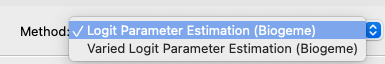
\includegraphics[width=12cm]{img/gui/processingwidget-dropdown.png}
  \caption{Generisches DropDown-Menü im \classref{ProcessingWidget}.}
  \label{gui:fig_processingwidget-dropdown}
\end{figure}

Die funktionalen Ausdrücke bieten dank Python eine generische Möglichkeit Objekte beliebiger Datentypen in die Ausdrücke einzusetzen. Das ist besonders hilfreich, da unterschiedliche Bibliotheken Spaltensbleitungen und Alternativen in unterschiedlichen Formaten benötigen könnten. Egal ob die Funktionen mit bestimmten Variablen-Objekten direkt im Python-Code definiert werden müssen (wie in \emph{Biogeme}) oder ob ein Syntaxbaum erforderlich ist; funktionale Ausdrücke bieten sind durch ihre einfache Struktur extrem vielseitig einsetzbar.\\

Das Interface \classref{Optimizer} ermöglicht die Implementierung von Verfahren, um ein definiertes Diskretes Wahlmodell auf Grundlage eines Ergebnisses zu optimieren.

\subsection{Benutzbarkeit}
%Fehlertolleranz

Die Anwendung bietet eine Reihe von Hilfsmitteln um den Nutzer bei der Bedienung zu unterstützen. Sie wird über eine intuitive Benutzeroberfläche bedient, mit der der Nutzer schrittweise durch das Programm geführt wird (Abbildung~\ref{gui:fig_columns+model}. Es existieren zusätzliche Hinweistexte um z.~B. die Funktion von Schaltflächen besser zu kommunizieren. Aussagekräftige Fehlermeldungen erklären dem Nutzer, was er falsch macht (Abbildung~\ref{gui:fig_error-dialog-example}).\\

\begin{figure}[H]%
  \centering
  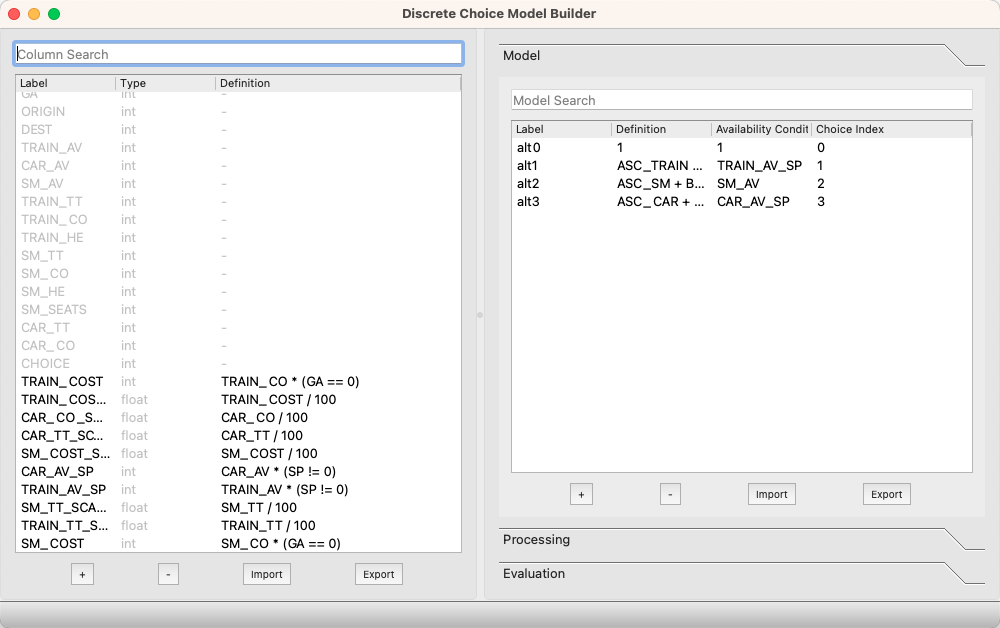
\includegraphics[width=12cm]{img/gui/columns+model.png}
  \caption{Hauptfenster mit Spaltenübersicht links und Modellverwaltung rechts}
  \label{gui:fig_columns+model}
\end{figure}

\begin{figure}[H]%
  \centering
  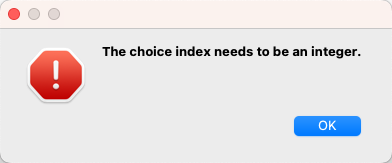
\includegraphics[width=12cm]{img/gui/error-dialog-example.png}
  \caption{Dialogfenster mit aussagekräftiger Fehlermeldung.}
  \label{gui:fig_error-dialog-example}
\end{figure}

Besonders Nutzerfreundlich ist die Fehlerkennzeichnung innerhalb von definierten Ausdrücken, wie sie z.~B. bei Spaltenableitungen oder Nutzenfunktionen vorkommen. Fehler werden direkt an der entscheidenden Stelle mit einer roten Hinterlegung hervorgehoben. Bewegt der Nutzer den Mauszeiger auf diese Markierung, erhält er eine Erklärung des Problems (Abbildung~\ref{gui:fig_expression-error-syntax}).\\

\begin{figure}[H]%
  \centering
  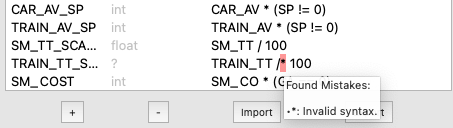
\includegraphics[width=12cm]{img/gui/expression-error-syntax.png}
  \caption{Rote Markierung eines Syntaxfehlers in einer Spaltenableitung.}
  \label{gui:fig_expression-error-syntax}
\end{figure}

In den Nutzertests wurde durch den Fragebogen die Kriterien der Benutzbarkeit evaluiert. Dabei wurde die Bedienbarkeit mit 81, die Verständlichkeit mit 52 und die Erlernbarkeit mit 81 von je 100 bewertet. Die niedrige Bewertung der Verständlichkeit hat die Qualitätssicherung maßgeblich beeinflusst und den Fokus auf die Verbesserung dessen gerichtet. Daher wurden eine Bedienungsanleitung (\emph{User Manual}), sowie die Erklärungen von Knöpfen und Syntax hinzugefügt. Daher ist davon auszugehen, dass das Programm verständlicher geworden ist.\\

Beim freien Feedback wurde die Benutzbarkeit durch die übersichtliche Gestaltung sowie das einfache Einfügen der Funktionen als positiv bewertet.

\subsection{Funktionalität}

Auch die Funktionalität wurde in den Nutzertests bewertet. Diese erzielte eine Bewertung von 74 aus 100. Die Nutzer haben dabei beurteilt, ob das Programm aus ihrer Sicht vollständig ist und alle gewünschten Funktionen enthält, sowie ob sie das Programm selbst verwenden würden oder weiterempfehlen würden um Diskrete Choice Modelle zu berechnen.\\

Im Allgemeinen waren die Nutzer zufrieden mit der Funktionalität, allerdings sind ihnen Funktionen eingefallen, die im Pflichtenheft nicht abgegrenzt wurden. Diese sind im Punkt \ref{usertests} aufgeführt worden.\\

In dem Feedback der Nutzertests, wurde die einfache Funktionalität des Programms ebenfalls durch wiedergespiegelt. So wurden insebsondere die automatische Typerkennung der Ableitungsfunktionen, die Fehlerlokalisierung in den Funktionen, die einfachen Imports und Exports von bereits existierenden Ableitungen und Alternativen als gute Funktionalität hervorgehoben.\\

\subsection{Effizienz}

In den Nutzertests wurde auch das Zeitverhalten des Programms bewertet, es erzielte 71 von 100. Als größter Zeitfaktor wurde dabei das Erlernen bemängelt, da die Nutzer angaben die Berechnungen seien als effizient empfunden worden, sie haben sich aber nicht effizient und schnell produktiv in der Bedienung des Programms wahrgenommen. Diese Erlernbarkeit wurde in der Qualitätssicherungsphase durch die Verbesserung der Verständlichkeit indirekt behoben.

\subsection{Zuverlässigkeit}

Zur Gewährleistung der Fehlertoleranz wurde sichergestellt, dass das Programm bei auftretenden Fehlern nicht abstürzt, sonder diese an den Nutzer übermittelt. Daher werden alle abgefangenen Exceptions durch eine Fehlermeldung dem Nutzer mitgeteilt.\\

Ebenfalls ist die Fehlertoleranz in den Funktionen sichergestellt, durch die Fehlermeldungen, wie bereits im obigen Abschnitt beschrieben.\\

Die Wiederherstallbarkeit ist ebenfalls gut. Der Speicherprozess wird nach jedem Schritt angestoßen, sofern nicht bereits ein anderer Speicherprozess läuft, oder der Nutzer keinen Speicherort vergeben hat. Das gespeicherte Projekt kann dann jederzeit geöffnet werden, und das Programm befindet sich im selben Zustand wie zum Zeitpunkt der Speicherung.\\


\section{Anhang} \label{anhang}
\subsection{Aufgaben für den Nutzer Test}
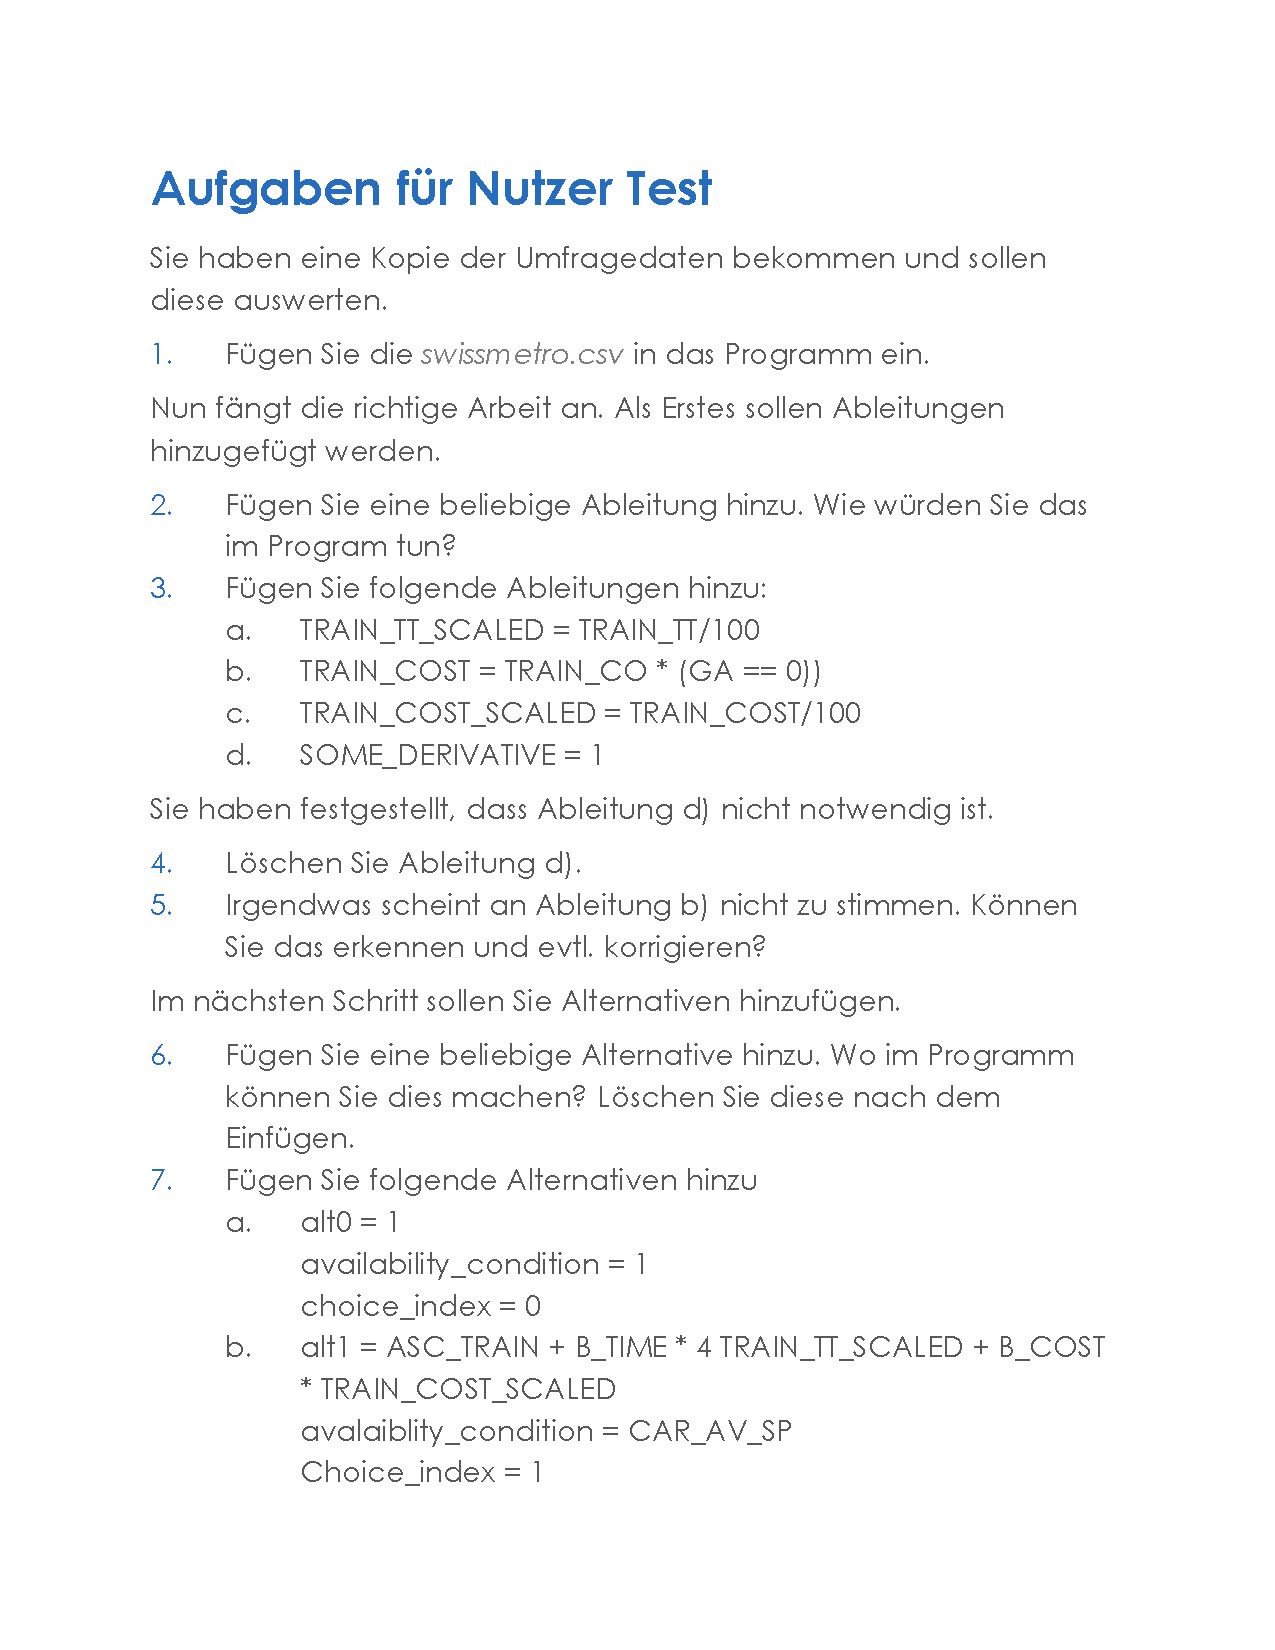
\includegraphics[width=1\textwidth,height=1\textheight]{ressources/aufgaben.pdf}
\newpage
\includegraphics[page = 2, width=1\textwidth,height=1\textheight]{ressources/aufgaben.pdf}
\subsection{Fragebogen für den Nutzer Test}
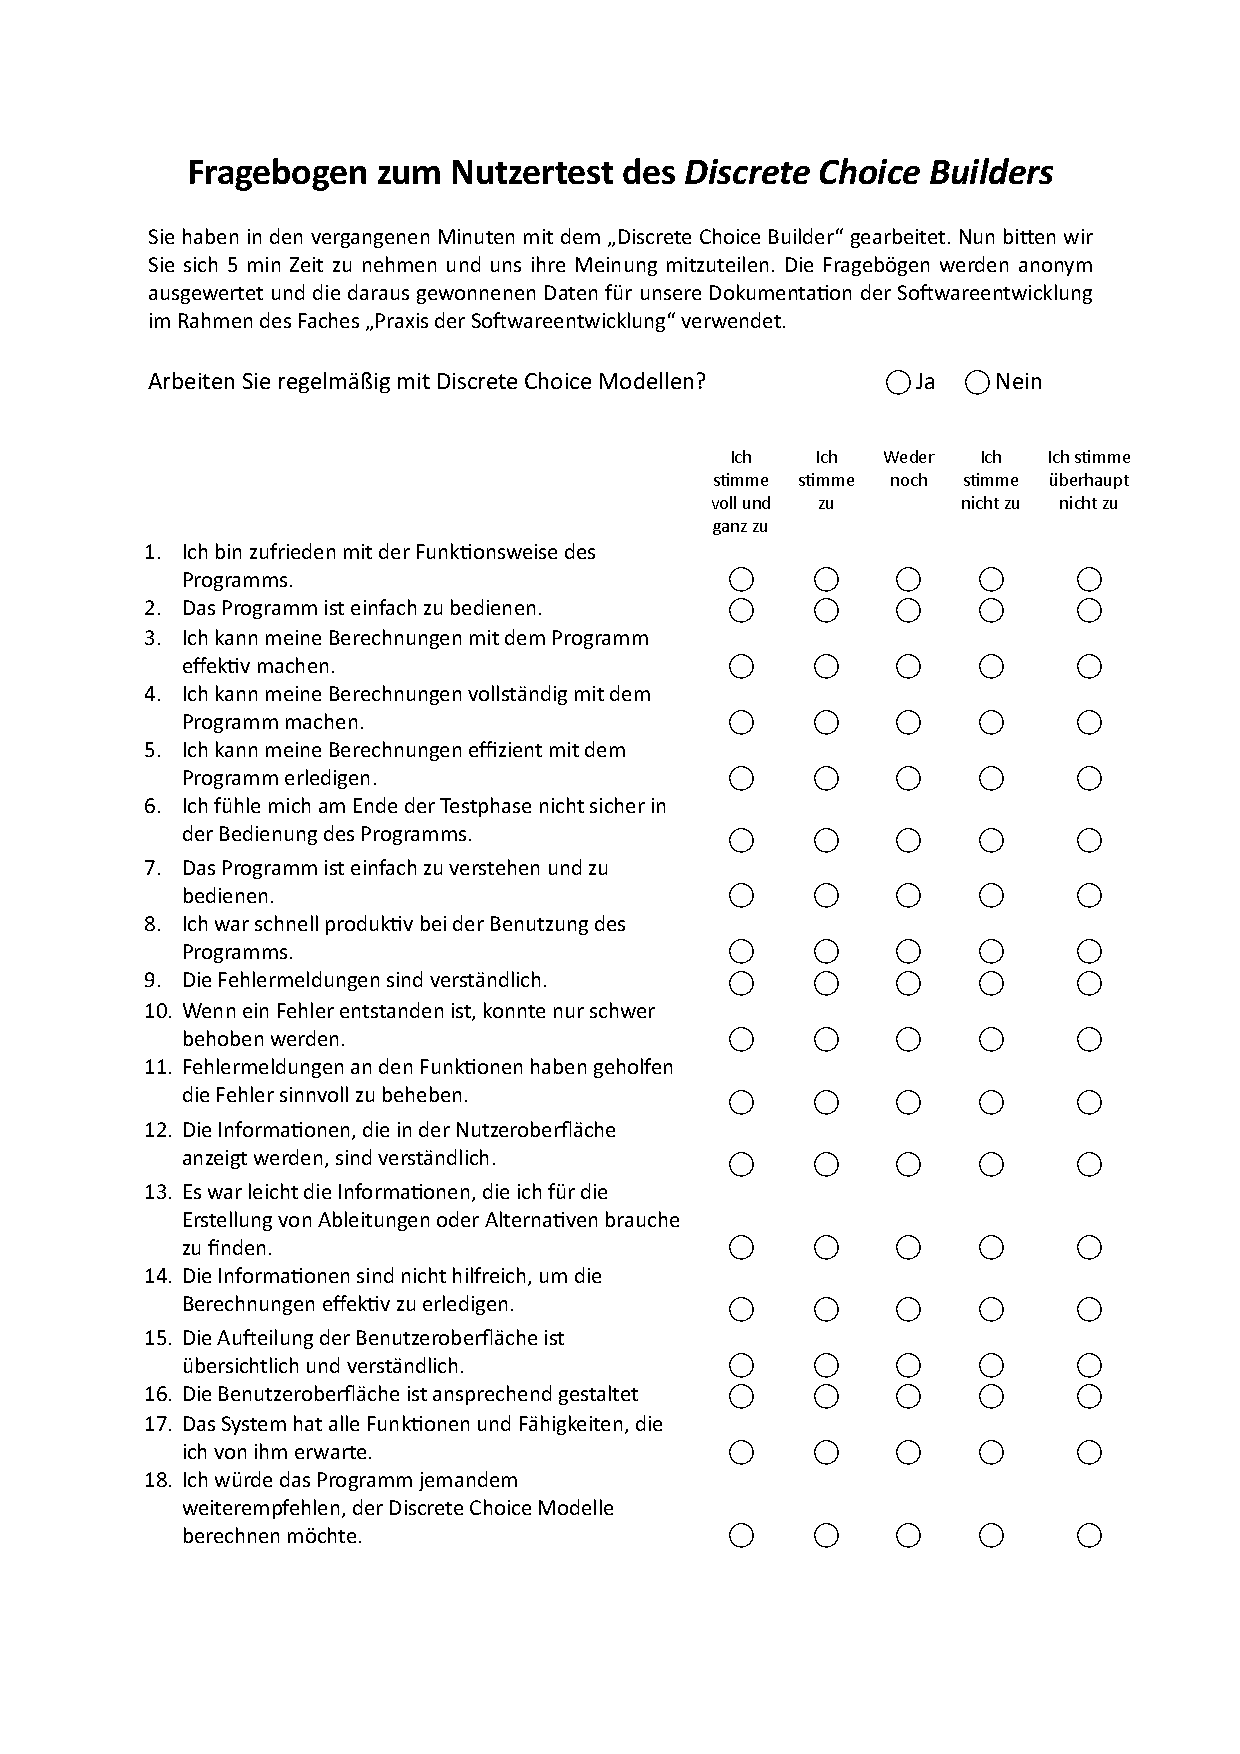
\includegraphics[width=1\textwidth,height=1\textheight]{ressources/NutzertestsFragebogen.pdf}
\newpage
\includegraphics[page = 2, width=1\textwidth,height=1\textheight]{ressources/NutzertestsFragebogen.pdf}
\newpage
\clearpage
\printunsrtglossary
%\printglossary
\end{document}